\documentclass[11pt]{article}
\usepackage[english]{babel}
\usepackage[paper=letterpaper, top=0.85in, bottom=1.0in, left=0.9in, right=0.9in, includehead, includefoot]{geometry}
\usepackage{amsmath,amssymb}
\usepackage{graphicx}
\usepackage{booktabs}
\usepackage{multirow}
\usepackage{xcolor}
\usepackage{tikz}
\usetikzlibrary{positioning,arrows.meta,calc,fit,backgrounds}
\usepackage{pgfplots}
\usepgfplotslibrary{groupplots,fillbetween}
\pgfplotsset{compat=1.18}
\usepackage{subcaption}
\usepackage{tabularx}
\usepackage{float}
\usepackage{enumitem}
\usepackage[colorlinks=true, allcolors=blue!50!black]{hyperref}
\usepackage{cleveref}
\linespread{1.08}

\newcommand{\best}[1]{\textbf{#1}}
\makeatletter\newcommand{\tabinput}[1]{\@@input #1 }\makeatother
% Shared pgfplots styles (colorblind-safe palette).
\definecolor{cPers}{HTML}{8C8C8C}
\definecolor{cSnaive}{HTML}{B07AA1}
\definecolor{cRidge}{HTML}{59A14F}
\definecolor{cYtwo}{HTML}{E15759}
\definecolor{cResid}{HTML}{F28E2B}
\definecolor{cFull}{HTML}{EDC948}
\definecolor{cYthree}{HTML}{4E79A7}
\pgfplotsset{
  y3base/.style={width=5.6cm, height=4.2cm, grid=major, grid style={gray!25},
    tick label style={font=\scriptsize}, label style={font=\scriptsize},
    title style={font=\footnotesize, yshift=-1ex}, legend style={font=\scriptsize}},
  mPers/.style={cPers, densely dotted, thick, mark=none},
  mSnaive/.style={cSnaive, dashdotted, thick, mark=none},
  mRidge/.style={cRidge, dashed, thick, mark=none},
  mYtwo/.style={cYtwo, thick, mark=o, mark size=1.2pt},
  mResid/.style={cResid, thick, mark=none},
  mFull/.style={cFull, thick, mark=none},
  mYthree/.style={cYthree, very thick, mark=square*, mark size=1.1pt},
}

% Generated by modeling/experiments/y3_audit_numbers.py. Do not edit.
\newcommand{\ReproOWMAE}{6.62}
\newcommand{\ReproOWRMSE}{24.14}
\newcommand{\ReproOWRtwo}{0.211}
\newcommand{\ReproSLMAE}{8.36}
\newcommand{\ReproSLRMSE}{14.84}
\newcommand{\ReproSLRtwo}{0.403}
\newcommand{\AuditPersLegacyHone}{56.7}
\newcommand{\AuditPersCausalHone}{62.2}
\newcommand{\AuditPersLegacyAvg}{62.3}
\newcommand{\AuditPersCausalAvg}{64.4}
\newcommand{\AuditPersHonePct}{9.7}
\newcommand{\ParamsDist}{468{,}511}
\newcommand{\ParamsResid}{449{,}592}
\newcommand{\ParamsYtwo}{449{,}592}

% Generated by modeling/experiments/y3_tables.py from results_y3/summary. Do not edit.
\newcommand{\ChgMAEOWDL}{-9.8}
\newcommand{\ChgEnsMAEOWDL}{-10.2}
\newcommand{\ChgRMSEOWDL}{-2.2}
\newcommand{\ChgEnsRMSEOWDL}{-2.3}
\newcommand{\ChgMISOWDL}{-19.0}
\newcommand{\ChgEnsMISOWDL}{-19.9}
\newcommand{\PICPOWDL}{0.949}
\newcommand{\PICPEnsOWDL}{0.949}
\newcommand{\PICPYtwoOWDL}{0.953}
\newcommand{\SkillYthreeEnsOWDL}{25.3}
\newcommand{\SkillRidgeOWDL}{22.5}
\newcommand{\ChgMAEOWUL}{-2.4}
\newcommand{\ChgEnsMAEOWUL}{-1.8}
\newcommand{\ChgRMSEOWUL}{0.4}
\newcommand{\ChgEnsRMSEOWUL}{-0.1}
\newcommand{\ChgMISOWUL}{-24.0}
\newcommand{\ChgEnsMISOWUL}{-26.3}
\newcommand{\PICPOWUL}{0.950}
\newcommand{\PICPEnsOWUL}{0.950}
\newcommand{\PICPYtwoOWUL}{0.952}
\newcommand{\SkillYthreeEnsOWUL}{22.8}
\newcommand{\SkillRidgeOWUL}{13.0}
\newcommand{\ChgMAESLDL}{-10.9}
\newcommand{\ChgEnsMAESLDL}{-14.6}
\newcommand{\ChgRMSESLDL}{-4.1}
\newcommand{\ChgEnsRMSESLDL}{-5.0}
\newcommand{\ChgMISSLDL}{-39.3}
\newcommand{\ChgEnsMISSLDL}{-41.1}
\newcommand{\PICPSLDL}{0.954}
\newcommand{\PICPEnsSLDL}{0.953}
\newcommand{\PICPYtwoSLDL}{0.950}
\newcommand{\SkillYthreeEnsSLDL}{45.3}
\newcommand{\SkillRidgeSLDL}{41.7}
\newcommand{\ChgMAESLUL}{-2.8}
\newcommand{\ChgEnsMAESLUL}{-3.3}
\newcommand{\ChgRMSESLUL}{0.1}
\newcommand{\ChgEnsRMSESLUL}{-0.1}
\newcommand{\ChgMISSLUL}{-8.4}
\newcommand{\ChgEnsMISSLUL}{-9.4}
\newcommand{\PICPSLUL}{0.935}
\newcommand{\PICPEnsSLUL}{0.936}
\newcommand{\PICPYtwoSLUL}{0.932}
\newcommand{\SkillYthreeEnsSLUL}{26.6}
\newcommand{\SkillRidgeSLUL}{25.9}
\newcommand{\ChgMAEQDL}{-1.5}
\newcommand{\ChgEnsMAEQDL}{-1.6}
\newcommand{\ChgRMSEQDL}{-1.0}
\newcommand{\ChgEnsRMSEQDL}{-1.0}
\newcommand{\ChgMISQDL}{-13.3}
\newcommand{\ChgEnsMISQDL}{-13.9}
\newcommand{\PICPQDL}{0.950}
\newcommand{\PICPEnsQDL}{0.950}
\newcommand{\PICPYtwoQDL}{0.953}
\newcommand{\SkillYthreeEnsQDL}{31.9}
\newcommand{\SkillRidgeQDL}{29.5}
\newcommand{\ChgMAEQUL}{-17.7}
\newcommand{\ChgEnsMAEQUL}{-17.8}
\newcommand{\ChgRMSEQUL}{-0.3}
\newcommand{\ChgEnsRMSEQUL}{-0.3}
\newcommand{\ChgMISQUL}{-28.1}
\newcommand{\ChgEnsMISQUL}{-28.3}
\newcommand{\PICPQUL}{0.949}
\newcommand{\PICPEnsQUL}{0.950}
\newcommand{\PICPYtwoQUL}{0.948}
\newcommand{\SkillYthreeEnsQUL}{29.1}
\newcommand{\SkillRidgeQUL}{29.1}
\newcommand{\ChgMAEBest}{-17.7}
\newcommand{\ChgMAEWorst}{-1.5}
\newcommand{\ChgMAEMean}{-7.5}
\newcommand{\ChgEnsMAEBest}{-17.8}
\newcommand{\ChgEnsMAEWorst}{-1.6}
\newcommand{\ChgEnsMAEMean}{-8.2}
\newcommand{\ChgRMSEBest}{-4.1}
\newcommand{\ChgRMSEWorst}{0.4}
\newcommand{\ChgRMSEMean}{-1.2}
\newcommand{\ChgEnsRMSEBest}{-5.0}
\newcommand{\ChgEnsRMSEWorst}{-0.1}
\newcommand{\ChgEnsRMSEMean}{-1.5}
\newcommand{\ChgMISBest}{-39.3}
\newcommand{\ChgMISWorst}{-8.4}
\newcommand{\ChgMISMean}{-22.0}
\newcommand{\ChgEnsMISBest}{-41.1}
\newcommand{\ChgEnsMISWorst}{-9.4}
\newcommand{\ChgEnsMISMean}{-23.2}
\newcommand{\PICPMin}{0.935}
\newcommand{\PICPMax}{0.954}
\newcommand{\PICPEnsMin}{0.936}
\newcommand{\PICPEnsMax}{0.953}
\newcommand{\RatioRMSEMAEMin}{1.5}
\newcommand{\RatioRMSEMAEMax}{3.8}
\newcommand{\AUCYtwoOWDL}{0.765}
\newcommand{\AUCYthreeOWDL}{0.732}
\newcommand{\AUCRidgeOWDL}{0.695}
\newcommand{\AUCPersOWDL}{0.652}
\newcommand{\AUCYtwoOWUL}{0.965}
\newcommand{\AUCYthreeOWUL}{0.961}
\newcommand{\AUCRidgeOWUL}{0.951}
\newcommand{\AUCPersOWUL}{0.936}
\newcommand{\AUCYtwoSLDL}{0.832}
\newcommand{\AUCYthreeSLDL}{0.901}
\newcommand{\AUCRidgeSLDL}{0.834}
\newcommand{\AUCPersSLDL}{0.699}
\newcommand{\AUCYtwoSLUL}{0.797}
\newcommand{\AUCYthreeSLUL}{0.809}
\newcommand{\AUCRidgeSLUL}{0.783}
\newcommand{\AUCPersSLUL}{0.749}
\newcommand{\AUCYtwoQDL}{0.792}
\newcommand{\AUCYthreeQDL}{0.795}
\newcommand{\AUCRidgeQDL}{0.792}
\newcommand{\AUCPersQDL}{0.599}
\newcommand{\AUCYtwoQUL}{0.594}
\newcommand{\AUCYthreeQUL}{0.607}
\newcommand{\AUCRidgeQUL}{0.607}
\newcommand{\AUCPersQUL}{0.514}
\newcommand{\InterpFracSLDL}{11.9}
\newcommand{\InterpFracSLUL}{1.2}
\newcommand{\RealMAEYtwoSLDL}{21.25}
\newcommand{\RealRMSEYtwoSLDL}{37.38}
\newcommand{\AllMAEYtwoSLDL}{21.60}
\newcommand{\AllRMSEYtwoSLDL}{37.13}
\newcommand{\RealMAEYthreeSLDL}{17.86}
\newcommand{\RealRMSEYthreeSLDL}{35.60}
\newcommand{\AllMAEYthreeSLDL}{18.45}
\newcommand{\AllRMSEYthreeSLDL}{35.31}
\newcommand{\TimeSSCPU}{6.9}
\newcommand{\TimeDSCPU}{10.0}
\newcommand{\JitISSLDLDS}{2.8}
\newcommand{\JitISSLDLS}{8.5}
\newcommand{\EpochsMin}{16}
\newcommand{\EpochsMax}{44}
\newcommand{\EpochsMedian}{24}
\newcommand{\NRuns}{72}
\newcommand{\BestEpochMax}{29}

% Generated by modeling/experiments/y3_report_tables2.py. Do not edit.
\newcommand{\BiasYtwoOWDL}{+6.8}
\newcommand{\BiasYthreeOWDL}{+3.17}
\newcommand{\BiasYtwoOWUL}{+4.9}
\newcommand{\BiasYthreeOWUL}{+4.52}
\newcommand{\BiasYtwoSLDL}{+2.2}
\newcommand{\BiasYthreeSLDL}{+0.59}
\newcommand{\BiasYtwoSLUL}{+1.1}
\newcommand{\BiasYthreeSLUL}{+0.08}
\newcommand{\BiasYtwoQDL}{+0.2}
\newcommand{\BiasYthreeQDL}{-0.12}
\newcommand{\BiasYtwoQUL}{+6.0}
\newcommand{\BiasYthreeQUL}{+0.19}
\newcommand{\RhoMin}{0.17}
\newcommand{\RhoMax}{0.64}
\newcommand{\SessWinsOWDL}{11}
\newcommand{\SessNOWDL}{11}
\newcommand{\SessPOWDL}{0.0010}
\newcommand{\SessWinsOWUL}{8}
\newcommand{\SessNOWUL}{11}
\newcommand{\SessPOWUL}{0.1475}
\newcommand{\SessWinsSLDL}{8}
\newcommand{\SessNSLDL}{9}
\newcommand{\SessPSLDL}{0.0078}
\newcommand{\SessWinsSLUL}{9}
\newcommand{\SessNSLUL}{9}
\newcommand{\SessPSLUL}{0.0039}
\newcommand{\SessWinsQDL}{48}
\newcommand{\SessNQDL}{58}
\newcommand{\SessPQDL}{10^{-4}}
\newcommand{\SessWinsQUL}{58}
\newcommand{\SessNQUL}{58}
\newcommand{\SessPQUL}{10^{-4}}
\newcommand{\SessWinsTotal}{142}
\newcommand{\SessNTotal}{156}


\begin{document}
\sloppy

\begin{titlepage}
  \noindent\begin{minipage}[t]{0.3\textwidth}
    \vspace{-1.5em}
    
\includegraphics[width=\linewidth,height=1.5cm,keepaspectratio]{figures/collins_logo.jpeg}%
  \end{minipage}%
  \hfill
  \begin{minipage}[t]{0.55\textwidth}
    \vspace{-1.5em}
    \raggedleft
    
\includegraphics[width=\linewidth,height=1.5cm,keepaspectratio]{figures/wici_log3.png}%
  \end{minipage}
  \centering
  \vspace*{\fill}
  {\LARGE\bfseries Collins Aerospace -- ISU WiCI \\[1em]
  Integrated Terrestrial and Satellite Communications (Year 3)\\[1em]
  Link-State Forecasting: Audit, Distributional Models,\\ and Calibrated Uncertainty\par}
  \vspace*{\fill}
  {\large
    ISU Personnel: Jalal Jalali, Evan Gossling, Daji Qiao, Hongwei Zhang\\
    Collins Personnel: Naveen Rajanikantha, Ben Haan, Andrew Bys \par}
  \vspace*{1em}
  {\large November 2026\par}
  \vspace*{\fill}
  {\normalsize Copyright \copyright{} 2026 Center for Wireless, Communities and Innovation (WiCI) \par}
\end{titlepage}

\tableofcontents
\newpage

% ==========================================================================
\section{Executive Summary}
This report covers the Year 3 work on forecasting the state of satellite and terrestrial links for the prediction-aware multipath client built in Year 2. The task is to predict the RTT, jitter, and packet loss of a Starlink, a OneWeb, and a 5G link from 0.2\,s to 3\,s ahead, from 6\,s of 5\,Hz measurements.

\paragraph{What we found in the Year 2 pipeline.} We reproduced the Year 2 results and audited the data and the evaluation (Section~\ref{sec:audit}). Six issues were found and fixed. Three of them change how the Year 2 numbers should be read:
\begin{itemize}[leftmargin=*]
  \item The Starlink parser fills missing server pings by interpolating toward the next real ping (\InterpFracSLDL\% of the downlink test targets). This leaks part of the future into the model input and makes Starlink RTT look easier to predict than it is.
  \item The Year 2 95\% interval coverage was computed from the test residuals themselves and is 0.95 by construction.
  \item The horizon steps are 200\,ms, not 1\,s. The Year 2 ``15\,s'' horizon is 3\,s.
\end{itemize}

\paragraph{What changed in Year 3.} Every method now uses causal inputs. The Year 3 forecaster keeps the Year 2 encoder and attention but anchors the decoder on the last observation, adds causal context features, and, most importantly, predicts a mean and five quantiles for every target and step instead of a single value. Intervals are calibrated on held-out sessions with conformalized quantile regression, and three seeds are combined into an ensemble.

\paragraph{Results (test sessions, 3 seeds, against the Year 2 model retrained on the same corrected data).}
\begin{itemize}[leftmargin=*]
  \item \textbf{Calibrated uncertainty:} the 95\% interval score of the RTT forecasts improves on all six links, by \ChgMISWorst\% to \ChgMISBest\% (mean \ChgMISMean\%), with measured coverage of \PICPMin--\PICPMax{} on unseen sessions. Jitter and loss intervals improve on every link as well.
  \item \textbf{Absolute error:} the RTT MAE drops on all six links, by \ChgMAEWorst\% to \ChgMAEBest\% (mean \ChgMAEMean\%). The gains are largest on the links with spiky RTT (5G UL \ChgMAEQUL\%, Starlink DL \ChgMAESLDL\%, OneWeb DL \ChgMAEOWDL\%).
  \item \textbf{Squared error:} RMSE and $R^2$ are essentially unchanged (RMSE \ChgRMSEBest\% to $+$\ChgRMSEWorst\%). We did not find a change that reliably lowers the RTT RMSE by more than a few percent. A tuned linear model reaches a similar RMSE skill as the Year 2 network on four of the six links.
\end{itemize}
The improvement is therefore not in the squared error of the point forecast, which appears close to what the 6\,s window can support, but in the robustness of the point forecast to RTT spikes and in calibrated, input-dependent uncertainty. For the multipath scheduler this means a per-path risk bound that is tighter when a path is calm and widens when it is about to become unstable.


% ==========================================================================
\section{Introduction}
Integrated terrestrial and low Earth orbit (LEO) satellite networks give an airborne or remote terminal several paths with very different behavior. A 5G link has low and fairly stable latency but limited coverage. Starlink and OneWeb links have global coverage but their round-trip time (RTT), jitter, and loss change quickly with satellite handovers, scheduler reconfigurations, and load~\cite{michel2022first,mohan2024multifaceted}. The Year 2 work of this project built a Multipath QUIC (MPQUIC) \emph{liquid tunnel} that combines these paths and showed that a scheduler fed with short-horizon forecasts of path state loses fewer video frames than a reactive minRTT scheduler~\cite{deconinck2017multipath}. The quality of those forecasts is therefore a direct input to the quality of the scheduling decisions.

The Year 2 Modeling Dynamics report compared eight forecasting models on six links (Starlink, OneWeb, and 5G, each in downlink and uplink) and selected a GRU sequence-to-sequence model with additive attention (Seq2Seq-GRU) as the primary model~\cite{cho2014learning,bahdanau2015neural}. This Year 3 report starts from that model and asks three questions.
\begin{enumerate}[leftmargin=*]
  \item \textbf{Are the Year 2 numbers right?} We re-implemented the evaluation, reproduced the Year 2 results, and audited the data and the metrics. Section~\ref{sec:audit} lists six issues. One of them, an interpolation step in the Starlink parser, leaks part of the next RTT sample into the model input. Another one makes the Year 2 interval coverage equal to 95\% by construction.
  \item \textbf{Can the forecasts be made better?} Section~\ref{sec:methods} describes the Year 3 changes: a causal data pipeline, a residual decoder anchored on the last observation, engineered context features, and, most importantly, distributional output heads that predict a mean and five quantiles per target and horizon.
  \item \textbf{Can the uncertainty be trusted?} The scheduler needs to know how wrong a forecast may be. We calibrate intervals with split conformal prediction on held-out sessions~\cite{lei2018distribution,romano2019conformalized} and report the coverage that is actually achieved on unseen test sessions.
\end{enumerate}

\paragraph{Related work.} Measurement studies explain why LEO link state changes quickly. Starlink reassigns users to satellites in globally synchronized 15\,s slots, which produces latency jumps~\cite{mohan2024multifaceted,tanveer2023making}. Its throughput varies from sub-second to diurnal scales~\cite{garcia2023multitimescale}. OneWeb latency changes at each satellite and gateway handover~\cite{zhao2025measuring}, which an earlier study on our testbed also observed~\cite{perrin2025measurement}. Learned prediction of link performance is established for cellular networks~\cite{narayanan2020lumos5g,mei2019realtime}. At sub-second resolution, however, simple predictors are hard to beat~\cite{basit2024predictability}. For LEO networks, Starlink throughput and latency have been predicted at coarse resolution~\cite{liu2025vivisecting,benghe2026horizon}. A concurrent preprint forecasts LEO link state with quantile bands~\cite{chi2026reading}. On the transport side, MPQUIC schedulers act on smoothed RTT estimates~\cite{paasch2014experimental,lim2017ecf}. Measured multipath sessions over Starlink and cellular paths suffer from the resulting mismatch~\cite{baltaci2023multipath}. Handover-aware or forecast-driven schedulers have been proposed~\cite{yang2024mams,maglione2025intelligent}. None of these works checks the causality of the input alignment or calibrates forecast uncertainty on unseen sessions, which are the two gaps this report addresses.

All methods are compared on the same session-level split as Year 2, with three training seeds per neural model, against four non-neural references (persistence, a one-second seasonal repeat, and two ridge regressions). Every number in this report is produced by the scripts listed in Appendix~\ref{app:repro} and is stored in \texttt{modeling/\allowbreak{}results\_\allowbreak{}y3/\allowbreak{}}.


% ==========================================================================
\section{System Model and Data}
\subsection{Measurement setup}
The data were collected on the ARA wireless living lab~\cite{islam2025design}. A client node is connected to a Starlink user terminal, a OneWeb user terminal, and a 5G network through a Quectel modem. During each session the node runs a ping stream at 5\,Hz to a server, an iperf3 UDP stream that reports throughput, jitter, and loss once per second, and collectors for terminal telemetry (Starlink dish state and satellite geometry, OneWeb SINR, elevation, azimuth and handover events, 5G RSRP, RSRQ and SINR) and local weather. The parsers align all sources on the ping time base, which gives one row every 200\,ms. Figure~\ref{fig:system} shows the setup and where the forecaster sits in the multipath client.

\begin{figure}[t]
  \centering
  \resizebox{0.82\linewidth}{!}{% System model: ARA measurement setup and prediction-aware multipath client.
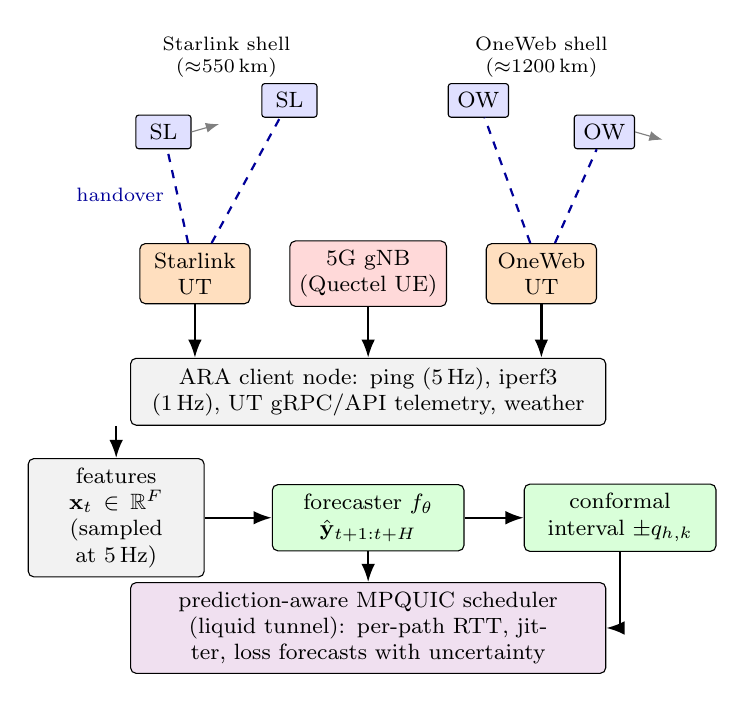
\begin{tikzpicture}[
  font=\footnotesize, >=Latex,
  sat/.style={draw, fill=blue!12, minimum width=7mm, minimum height=4mm, rounded corners=1pt},
  ut/.style={draw, fill=orange!25, minimum width=14mm, minimum height=6mm, align=center, rounded corners=2pt},
  blk/.style={draw, fill=gray!10, minimum height=7mm, align=center, rounded corners=2pt, text width=20mm},
  pred/.style={draw, fill=green!15, minimum height=7mm, align=center, rounded corners=2pt, text width=22mm},
  lnk/.style={->, thick},
  wl/.style={dashed, thick, blue!60!black}
]
% Satellites
\node[sat] (s1) at (0,4.2) {SL};
\node[sat] (s2) at (1.6,4.6) {SL};
\node[sat] (o1) at (4.0,4.6) {OW};
\node[sat] (o2) at (5.6,4.2) {OW};
\node[font=\scriptsize, align=center] at (0.8,5.15) {Starlink shell\\($\approx$550\,km)};
\node[font=\scriptsize, align=center] at (4.8,5.15) {OneWeb shell\\($\approx$1200\,km)};
\draw[->, gray] (s1.east) -- ++(0.35,0.1);
\draw[->, gray] (o2.east) -- ++(0.35,-0.1);
% UTs and gNB
\node[ut] (sut) at (0.4,2.4) {Starlink\\UT};
\node[ut] (out) at (4.8,2.4) {OneWeb\\UT};
\node[ut, fill=red!15] (gnb) at (2.6,2.4) {5G gNB\\(Quectel UE)};
\draw[wl] (sut) -- (s1); \draw[wl] (sut) -- (s2);
\draw[wl] (out) -- (o1); \draw[wl] (out) -- (o2);
\node[font=\scriptsize, blue!60!black] at (-0.55,3.4) {handover};
% Client node
\node[blk, text width=58mm, minimum height=8mm] (client) at (2.6,0.9) {ARA client node: ping (5\,Hz), iperf3 (1\,Hz), UT gRPC/API telemetry, weather};
\draw[lnk] (sut) -- (sut |- client.north);
\draw[lnk] (gnb) -- (client);
\draw[lnk] (out) -- (out |- client.north);
% Pipeline
\node[blk] (feat) at (-0.6,-0.7) {features $\mathbf{x}_t\in\mathbb{R}^{F}$\\(sampled at 5\,Hz)};
\node[pred] (model) at (2.6,-0.7) {forecaster $f_\theta$\\$\hat{\mathbf{y}}_{t+1:t+H}$};
\node[pred] (cp) at (5.8,-0.7) {conformal\\interval $\pm q_{h,k}$};
\draw[lnk] (client.south -| feat) -- (feat);
\draw[lnk] (feat) -- (model);
\draw[lnk] (model) -- (cp);
\node[blk, text width=58mm, fill=violet!12] (sched) at (2.6,-2.1) {prediction-aware MPQUIC scheduler (liquid tunnel): per-path RTT, jitter, loss forecasts with uncertainty};
\draw[lnk] (cp.south) |- (sched.east);
\draw[lnk] (model.south) -- (sched.north);
\end{tikzpicture}
}
  \caption{System model. Three access links are measured in parallel on the ARA client node. The forecaster maps a window of link-state features to a distribution of future RTT, jitter, and loss, which a conformal step turns into calibrated intervals for the prediction-aware MPQUIC scheduler.}
  \label{fig:system}
\end{figure}

Figure~\ref{fig:sysdetail} gives a more detailed view of the three planes of the system: the network and measurement plane, the data and forecasting plane developed in this report, and the scheduling plane that consumes the forecasts.

\begin{figure}[p]
  \centering
  \rotatebox{90}{\resizebox{0.95\textheight}{!}{% Detailed system model: network and measurement plane, data and forecasting plane, scheduling plane.
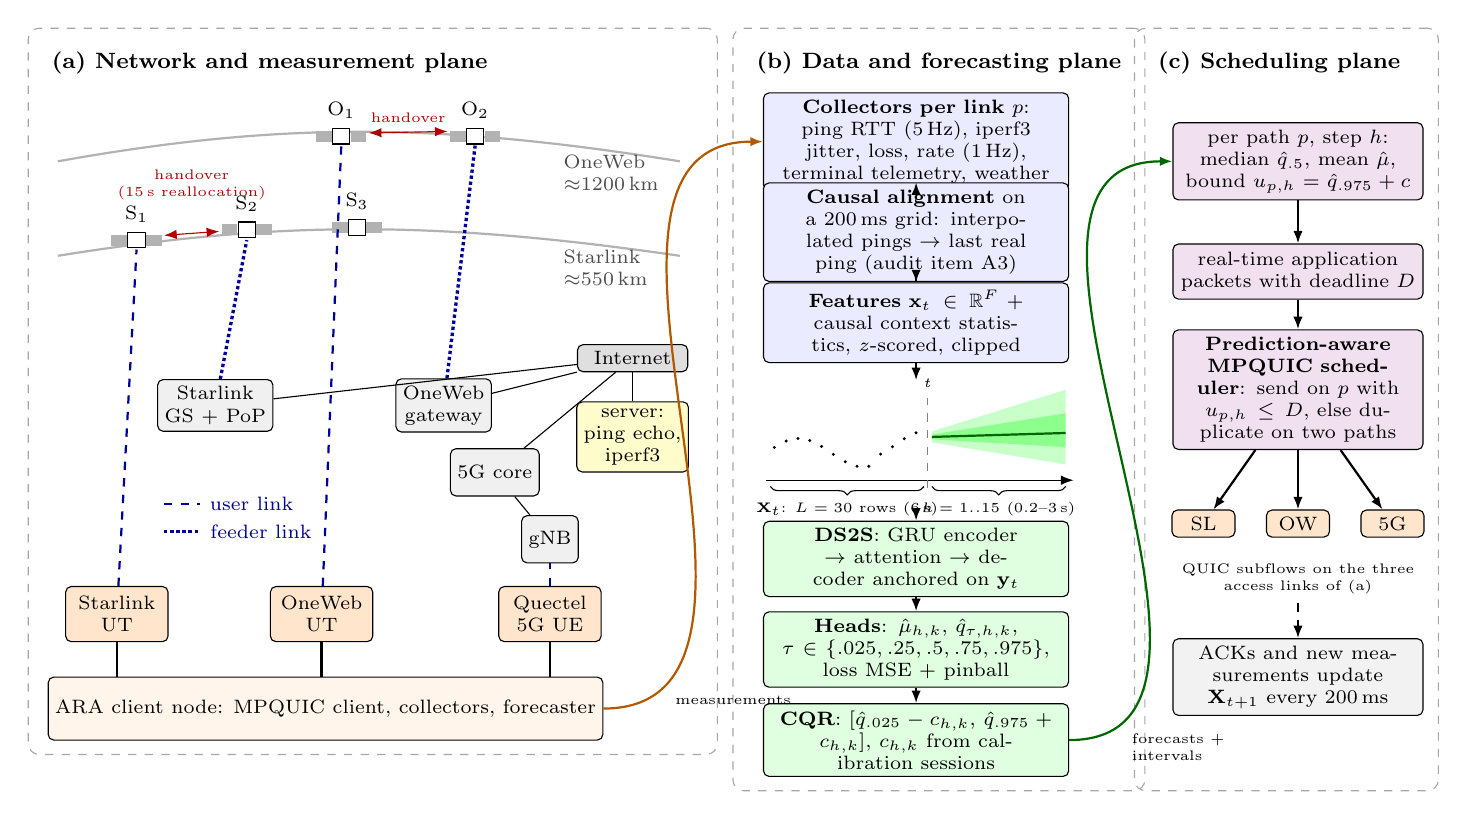
\begin{tikzpicture}[
  font=\scriptsize, >={Latex[length=1.6mm]},
  sat/.pic={\fill[gray!60] (-0.32,-0.07) rectangle (-0.12,0.07); \fill[gray!60] (0.12,-0.07) rectangle (0.32,0.07);
            \filldraw[fill=white, draw=black] (-0.11,-0.1) rectangle (0.11,0.1);},
  box/.style={draw, rounded corners=2pt, align=center, inner sep=2.5pt},
  gnd/.style={box, fill=gray!12, minimum height=6mm},
  ue/.style={box, fill=orange!20, minimum width=13mm, minimum height=7mm},
  pstep/.style={box, fill=blue!8, text width=37mm, minimum height=7mm},
  fstep/.style={box, fill=green!12, text width=37mm, minimum height=7mm},
  sch/.style={box, fill=violet!12, text width=30mm, minimum height=7mm},
  panel/.style={draw=gray!70, dashed, rounded corners=4pt, inner sep=5pt},
  ptitle/.style={font=\footnotesize\bfseries},
  ul/.style={dashed, thick, blue!60!black},
  fl/.style={densely dotted, very thick, blue!60!black},
  wl/.style={thick, ->}
]
% ===================== (a) network and measurement plane =====================
\node[ptitle, anchor=west] (ta) at (-0.5,8.75) {(a) Network and measurement plane};
\draw[gray!60, thick] (-0.3,6.3) .. controls (2.5,6.75) and (4.5,6.75) .. (7.6,6.3);
\draw[gray!60, thick] (-0.3,7.5) .. controls (2.5,8.0) and (4.5,8.0) .. (7.6,7.5);
\node[gray!60!black, anchor=west, align=left] at (6.0,6.15) {Starlink\\$\approx$550\,km};
\node[gray!60!black, anchor=west, align=left] at (6.0,7.35) {OneWeb\\$\approx$1200\,km};
\pic at (0.7,6.5) {sat}; \pic at (2.1,6.63) {sat}; \pic at (3.5,6.66) {sat};
\pic at (3.3,7.82) {sat}; \pic at (5.0,7.82) {sat};
\node at (0.7,6.83) {S$_1$}; \node at (2.1,6.96) {S$_2$}; \node at (3.5,6.99) {S$_3$};
\node at (3.3,8.15) {O$_1$}; \node at (5.0,8.15) {O$_2$};
\draw[<->, red!70!black] (1.05,6.56) -- (1.75,6.61);
\node[red!70!black, font=\tiny, align=center] at (1.4,7.2) {handover\\(15\,s reallocation)};
\draw[<->, red!70!black] (3.65,7.86) -- (4.65,7.88) node[midway, above, font=\tiny] {handover};
% ground segment
\node[gnd] (gs) at (1.7,4.4) {Starlink\\GS + PoP};
\node[gnd] (gw) at (4.6,4.4) {OneWeb\\gateway};
\node[gnd] (core) at (5.25,3.55) {5G core};
\node[box, fill=gray!25, minimum width=14mm] (inet) at (7.0,5.0) {Internet};
\node[box, fill=yellow!20] (srv) at (7.0,4.0) {server:\\ping echo,\\iperf3};
\draw[fl] (gs) -- (2.1,6.5);
\draw[fl] (gw) -- (5.0,7.7);
\draw (gs) -- (inet); \draw (gw) -- (inet); \draw (core) -- (inet); \draw (inet) -- (srv);
% user side
\node[ue] (sut) at (0.45,1.75) {Starlink\\UT};
\node[ue] (out) at (3.05,1.75) {OneWeb\\UT};
\node[ue] (qe) at (5.95,1.75) {Quectel\\5G UE};
\node[gnd] (gnb) at (5.95,2.7) {gNB};
\draw[ul] (sut) -- (0.7,6.38);
\draw[ul] (out) -- (3.3,7.7);
\draw[ul] (qe) -- (gnb); \draw (gnb) -- (core);
\node[box, fill=orange!8, minimum width=70mm, minimum height=8mm] (cn) at (3.1,0.55) {ARA client node: MPQUIC client, collectors, forecaster};
\draw[thick] (sut) -- (sut |- cn.north); \draw[thick] (out) -- (out |- cn.north); \draw[thick] (qe) -- (qe |- cn.north);
\draw[ul] (1.05,3.15) -- (1.5,3.15) node[right] {user link};
\draw[fl] (1.05,2.8) -- (1.5,2.8) node[right] {feeder link};
\node[panel, fit={(ta)(cn)(srv)(sut)(7.9,8.2)}] {};

% ===================== (b) data and forecasting plane =====================
\node[ptitle, anchor=west] (tb) at (8.45,8.75) {(b) Data and forecasting plane};
\node[pstep] (col) at (10.6,7.75) {\textbf{Collectors per link $p$}: ping RTT (5\,Hz), iperf3 jitter, loss, rate (1\,Hz), terminal telemetry, weather};
\node[pstep] (ali) at (10.6,6.6) {\textbf{Causal alignment} on a 200\,ms grid: interpolated pings $\rightarrow$ last real ping (audit item A3)};
\node[pstep] (feat) at (10.6,5.45) {\textbf{Features} $\mathbf{x}_t\in\mathbb{R}^F$ + causal context statistics, $z$-scored, clipped};
\begin{scope}[shift={(8.7,3.45)}]
  \draw[->] (0,0) -- (3.9,0);
  \foreach \x in {0.1,0.25,...,2.0} \fill[black] (\x,{0.35+0.18*sin(220*\x)+0.1*(\x>1.3)}) circle (0.6pt);
  \draw[decorate, decoration={brace, amplitude=3pt, mirror}] (0.05,-0.08) -- (2.0,-0.08) node[midway, below=2pt, font=\tiny] {$\mathbf{X}_t$: $L=30$ rows (6\,s)};
  \draw[dashed, gray] (2.05,-0.1) -- (2.05,1.05) node[above, font=\tiny, black] {$t$};
  \fill[green!30, opacity=0.7] (2.1,0.48) -- (3.8,0.2) -- (3.8,1.15) -- (2.1,0.62) -- cycle;
  \fill[green!55, opacity=0.7] (2.1,0.52) -- (3.8,0.42) -- (3.8,0.85) -- (2.1,0.58) -- cycle;
  \draw[green!40!black, thick] (2.1,0.55) -- (3.8,0.6);
  \draw[decorate, decoration={brace, amplitude=3pt, mirror}] (2.1,-0.08) -- (3.8,-0.08) node[midway, below=2pt, font=\tiny] {$h=1..15$ (0.2--3\,s)};
\end{scope}
\node[fstep] (enc) at (10.6,2.45) {\textbf{DS2S}: GRU encoder $\rightarrow$ attention $\rightarrow$ decoder anchored on $\mathbf{y}_t$};
\node[fstep] (head) at (10.6,1.3) {\textbf{Heads}: $\hat\mu_{h,k}$, $\hat q_{\tau,h,k}$, $\tau\in\{.025,.25,.5,.75,.975\}$, loss MSE + pinball};
\node[fstep] (cqr) at (10.6,0.15) {\textbf{CQR}: $[\hat q_{.025}-c_{h,k},\,\hat q_{.975}+c_{h,k}]$, $c_{h,k}$ from calibration sessions};
\draw[wl] (col) -- (ali); \draw[wl] (ali) -- (feat); \draw[wl] (feat) -- (10.6,4.72); \draw[wl] (10.6,3.05) -- (enc);
\draw[wl] (enc) -- (head); \draw[wl] (head) -- (cqr);
\node[panel, fit={(tb)(col)(cqr)(8.55,3.0)(12.65,3.0)}] {};
\draw[wl, orange!70!black] (cn.east) to[out=0, in=180] node[pos=0.12, below right, font=\tiny, black] {measurements} (col.west);

% ===================== (c) scheduling plane =====================
\node[ptitle, anchor=west] (tc) at (13.55,8.75) {(c) Scheduling plane};
\node[sch] (fc) at (15.45,7.5) {per path $p$, step $h$: median $\hat q_{.5}$, mean $\hat\mu$, bound $u_{p,h}=\hat q_{.975}+c$};
\node[sch] (app) at (15.45,6.1) {real-time application packets with deadline $D$};
\node[sch] (dec) at (15.45,4.6) {\textbf{Prediction-aware MPQUIC scheduler}: send on $p$ with $u_{p,h}\le D$, else duplicate on two paths};
\node[box, fill=orange!20, minimum width=8mm] (p1) at (14.25,2.9) {SL};
\node[box, fill=orange!20, minimum width=8mm] (p2) at (15.45,2.9) {OW};
\node[box, fill=orange!20, minimum width=8mm] (p3) at (16.65,2.9) {5G};
\draw[wl] (fc) -- (app); \draw[wl] (app) -- (dec);
\draw[wl] (dec) -- (p1); \draw[wl] (dec) -- (p2); \draw[wl] (dec) -- (p3);
\node[align=center, font=\tiny] (sf) at (15.45,2.2) {QUIC subflows on the three\\access links of (a)};
\node[sch, fill=gray!10] (fb) at (15.45,0.95) {ACKs and new measurements update $\mathbf{X}_{t+1}$ every 200\,ms};
\draw[wl, dashed] (sf) -- (fb);
\node[panel, fit={(tc)(fc)(fb)(p1)(p3)(cqr.south -| fb.south)}] {};
\draw[wl, green!40!black] (cqr.east) to[out=0, in=180] node[pos=0.1, below right, font=\tiny, black, align=left] {forecasts +\\intervals} (fc.west);
\end{tikzpicture}
}}
  \caption{Detailed system model. (a) Network and measurement plane: Starlink (about 550\,km, user reallocation every 15\,s), OneWeb (about 1200\,km, bent pipe), and 5G paths from the ARA client node to the measurement server. (b) Data and forecasting plane: causal alignment, feature window, distributional forecaster, and CQR calibration. (c) Scheduling plane: per-path forecasts and calibrated bounds drive the prediction-aware MPQUIC scheduler, and new measurements update the window every 200\,ms.}
  \label{fig:sysdetail}
\end{figure}

\subsection{Forecasting problem}
For a link, let $\mathbf{x}_t\in\mathbb{R}^{F}$ be the feature vector at row $t$ and $\mathbf{y}_t\in\mathbb{R}^{K}$ the $K=3$ targets (RTT in ms, iperf jitter in ms, iperf loss in \%). Given the window $\mathbf{X}_t=(\mathbf{x}_{t-L+1},\dots,\mathbf{x}_t)$ with $L=30$ rows, the model predicts $\mathbf{y}_{t+h}$ for $h=1,\dots,H$ with $H=15$. Because rows are 200\,ms apart, the input covers 6\,s of history and the horizon spans 0.2\,s to 3\,s. The Year 2 report labeled the horizon steps as seconds (\texttt{t+1s} to \texttt{t+15s}). They are steps of 200\,ms, which matters when the forecasts are matched to scheduler time constants.

\subsection{Datasets}
Table~\ref{tab:data} lists the six datasets. Sessions (one CSV file each) are split 70/15/15 into training, validation, and test sets by a random permutation with seed 42, exactly as in Year 2. All windows from one session therefore stay in one split, and the test sessions are never seen during training, model selection, or calibration.

\begin{table}[t]
\centering
\caption{Datasets. Windows are 30 input rows plus 15 target rows at 5\,Hz. For 5G, every fourth training window is used (Section~\ref{sec:protocol}). Features: Year 2 set / Year 3 set.}
\label{tab:data}
\small
\begin{tabular}{lrrrrrr}
\toprule
Link & Sessions (tr/va/te) & Train windows & Val windows & Test windows & Features \\
\midrule
OneWeb DL   & 45 / 9 / 11   & 117{,}558 & 22{,}655  & 27{,}492  & 9 / 31 \\
OneWeb UL   & 45 / 9 / 11   & 115{,}847 & 22{,}751  & 28{,}125  & 9 / 31 \\
Starlink DL & 37 / 7 / 9    & 105{,}906 & 20{,}025  & 25{,}838  & 19 / 41 \\
Starlink UL & 37 / 7 / 9    & 106{,}165 & 20{,}090  & 25{,}666  & 19 / 41 \\
5G DL       & 266 / 57 / 58 & 194{,}725$^\dagger$ & 166{,}266 & 169{,}204 & 10 / 32 \\
5G UL       & 265 / 56 / 58 & 193{,}502$^\dagger$ & 162{,}894 & 168{,}519 & 10 / 32 \\
\bottomrule
\end{tabular}

\smallskip
\footnotesize $^\dagger$ after keeping every fourth window (778{,}898 and 774{,}006 before subsampling).
\end{table}


% ==========================================================================
\section{Audit of the Year 2 Pipeline}
\label{sec:audit}
Before changing any model we rebuilt the Year 2 evaluation in a single script (\texttt{experiments/\allowbreak y3\_benchmark.py}) that loads the data with the Year 2 functions, uses the same session split, and trains the Year 2 Seq2Seq-GRU with the Year 2 optimizer settings. With the original data it reproduces the Year 2 Starlink DL result (MAE \ReproSLMAE, RMSE \ReproSLRMSE, $R^2$ \ReproSLRtwo, against 8.55, 14.95, and 0.406 in the Year 2 report) and the OneWeb DL result (MAE \ReproOWMAE, RMSE \ReproOWRMSE, $R^2$ \ReproOWRtwo, against 6.12, 23.73, and 0.217). The small gaps are within the seed-to-seed spread reported in Section~\ref{sec:results}. The script was then reviewed by three independent reviewers, each finding was checked by two further reviewers who tried to refute it, and the surviving findings were fixed. Table~\ref{tab:audit} summarizes them.

\begin{table}[t]
\centering
\caption{Issues found in the Year 2 pipeline and how Year 3 handles them.}
\label{tab:audit}
\small
\begin{tabularx}{\linewidth}{>{\raggedright\arraybackslash}p{3.6cm}X>{\raggedright\arraybackslash}p{3.8cm}}
\toprule
Issue & Effect on Year 2 numbers & Year 3 handling \\
\midrule
A1. Horizon unit & Steps of 200\,ms were labeled as seconds. The ``15\,s'' horizon is 3\,s. & Horizons reported as $h\times 0.2$\,s. \\
A2. Interval coverage & Intervals were built from quantiles of the \emph{test} residuals. PICP$_{95}$ is therefore 0.95 by construction and says nothing about calibration. & Split conformal intervals calibrated on validation sessions, coverage measured on test sessions. \\
A3. Starlink RTT interpolation & The parser fills missing server pings by time interpolation toward the \emph{next} real ping. In the test sessions \InterpFracSLDL\% of the Starlink DL and \InterpFracSLUL\% of the UL RTT targets are interpolated. The last input row can then contain part of the first target. & Interpolated inputs replaced by the last real ping for every method. Targets keep the measured series. \\
A4. Constant targets & OneWeb UL jitter and loss are zero in every row. Year 2 reported $R^2=1$ and MAE 0 for them and averaged these into the aggregate. & $R^2$ undefined for constant targets and left out of averages. Per-target results reported. \\
A5. ``Relative RMSE'' & The Year 2 persistence ratio compared the model with a lag-1 shift of the flattened multi-target, multi-horizon series, not with a persistence forecast. Values above 1 for OneWeb did not mean the model was worse than persistence. & Skill against a proper persistence forecast $\hat{y}_{t+h}=y_t$ for each target and horizon. \\
A6. One seed & Each model was trained once. The OneWeb UL Seq2Seq MAE differs between the report (22.81) and the stored run (23.93). & Three seeds per neural model, mean $\pm$ standard deviation, and seed ensembles. \\
\bottomrule
\end{tabularx}
\end{table}

\paragraph{Effect of A3.} Replacing the interpolated inputs raises the Starlink DL persistence RTT error at the first step by \AuditPersHonePct\%, from \AuditPersLegacyHone\,ms to \AuditPersCausalHone\,ms RMSE and the average over the horizon from \AuditPersLegacyAvg\,ms to \AuditPersCausalAvg\,ms. Every method that reads the last RTT value benefits from the leak, including the Year 2 model. All Year 3 comparisons therefore use the corrected inputs for every method, and the Year 2 model is retrained on them. The Year 2 report numbers for Starlink RTT are optimistic by a few percent at short horizons. The 5G and OneWeb RTT series have no interpolated values (all values lie on the ping resolution grid).

\paragraph{Other observations.} The iperf3 collector stamps each one-second report at the start of its interval, and the parsers snap it to the nearest ping row. An iperf value at row $t$ can therefore describe traffic up to about one second after $t$. The same alignment is used for every method and in Year 2. It mainly affects the jitter and loss inputs, which are also targets and are shifted consistently. We keep it for comparability and list it as a limitation (Section~\ref{sec:limits}).


% ==========================================================================
\section{Year 3 Methods}
\label{sec:methods}
The Year 3 forecaster is built in four steps. Each step is evaluated separately in Section~\ref{sec:results} so that its contribution can be seen.

\subsection{Step 1: residual decoder}
The Year 2 decoder starts every forecast from a zero vector and predicts the level of each target directly. Year 3 starts the decoder from the last observed target values $\mathbf{y}_t$ (read from the input window) and lets each head predict the change,
\begin{equation}
\hat{\mathbf{y}}_{t+h} = \hat{\mathbf{y}}_{t+h-1} + g_\theta(\mathbf{s}_h), \qquad \hat{\mathbf{y}}_{t} = \mathbf{y}_t ,
\label{eq:resid}
\end{equation}
where $\mathbf{s}_h$ is the decoder state at step $h$. With $g_\theta\equiv 0$ the model is exactly the persistence forecast. The network only has to learn the departure from it. Teacher forcing is applied per sample instead of per batch, and gradients flow through the fed-back predictions~\cite{bengio2015scheduled}. This step was already in the repository at the start of Year 3 but had not been evaluated.

\subsection{Step 2: causal data pipeline and context features}
\begin{itemize}[leftmargin=*]
  \item \textbf{Causal ping inputs} (audit item A3, applied to every method).
  \item \textbf{Sentinel removal.} Some 5G files contain logger sentinels (for example SINR $=-32768$). Radio values outside physical ranges (SINR in $[-50,60]$\,dB, RSRP in $[-160,-20]$\,dBm, RSRQ in $[-40,0]$\,dB) are set to missing and forward filled.
  \item \textbf{Context features.} For each target we add seven causal statistics computed per session: the number of rows since the value last changed (the phase inside the report cycle, since jitter and loss are one-second iperf reports held for five rows), the mean and maximum over the last second, the means over the last 30\,s and 60\,s, the standard deviation over the last 60\,s, and the session-to-date mean. We also add the time since the previous row, since collector gaps often precede RTT spikes. The 30-row window covers only 6\,s, and these features give the model a longer view at no extra sequence length.
  \item \textbf{Input clipping.} After $z$-scoring with training statistics, non-target inputs are clipped to $[-5,5]$. Heavy tails reach $|z|\approx 100$ and otherwise dominate the GRU input.
\end{itemize}

\subsection{Step 3: distributional output heads}
Link-state targets are heavy tailed. In the test sessions the RTT RMSE of the retrained Year 2 model is \RatioRMSEMAEMin{} to \RatioRMSEMAEMax{} times its MAE, against about 1.25 for Gaussian errors. A model trained only with squared error learns the conditional mean, which minimizes RMSE but is not the best forecast under absolute error, and it says nothing about how uncertain each forecast is. Each scoring function has its own optimal point forecast: the mean for squared error and the median for absolute error~\cite{gneiting2011making}. Year 3 therefore replaces each scalar head by a head with six outputs per target and step: a mean $\hat{\mu}$ and the quantiles $\hat{q}_\tau$ for $\tau\in\mathcal{T}=\{0.025, 0.25, 0.5, 0.75, 0.975\}$. All outputs are anchored on the last value as in~\eqref{eq:resid}, and the decoder feeds back its mean. The quantiles are built as the median plus or minus cumulative softplus gaps, which rules out quantile crossing,
\begin{equation}
\hat{q}_{0.25}=\hat{q}_{0.5}-\varsigma(a_1),\quad \hat{q}_{0.025}=\hat{q}_{0.25}-\varsigma(a_2),\quad
\hat{q}_{0.75}=\hat{q}_{0.5}+\varsigma(b_1),\quad \hat{q}_{0.975}=\hat{q}_{0.75}+\varsigma(b_2),
\end{equation}
with $\varsigma(u)=\log(1+e^u)$. The training loss on normalized targets is
\begin{equation}
\mathcal{L} = \frac{1}{NHK}\sum_{n,h,k}\Big[\big(\hat{\mu}_{nhk}-y_{nhk}\big)^2 + \frac{1}{|\mathcal{T}|}\sum_{\tau\in\mathcal{T}}\rho_\tau\big(y_{nhk}-\hat{q}_{\tau,nhk}\big)\Big],
\qquad \rho_\tau(e)=\max\{\tau e,(\tau-1)e\},
\label{eq:loss}
\end{equation}
where $\rho_\tau$ is the pinball loss of quantile regression~\cite{koenker1978regression}. The mean is used for RMSE and $R^2$ and the median for MAE. The extra cost is small: the distributional model has \ParamsDist{} parameters against \ParamsResid{} for the Step 1 model on OneWeb DL. Figure~\ref{fig:arch} shows the resulting architecture.

\begin{figure}[t]
  \centering
  \resizebox{0.86\linewidth}{!}{% Year 3 forecaster: GRU encoder, additive attention, residual autoregressive decoder.
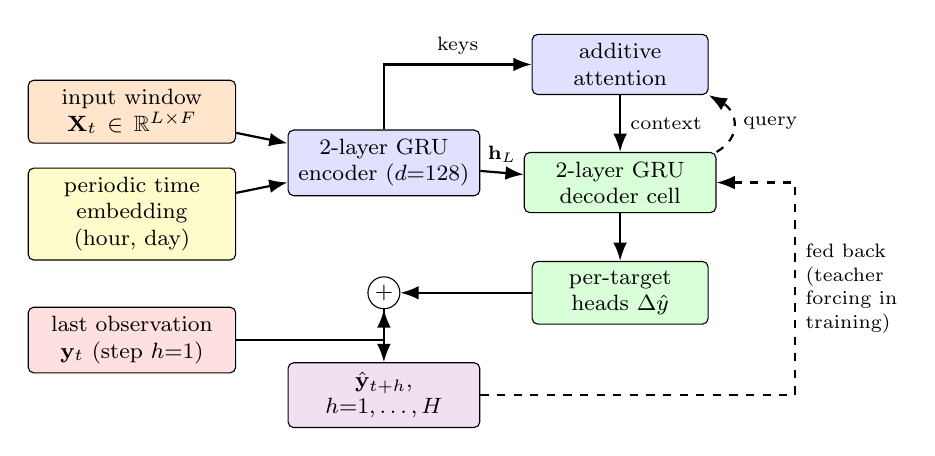
\begin{tikzpicture}[
  font=\footnotesize, >=Latex,
  b/.style={draw, rounded corners=2pt, minimum height=7mm, align=center, fill=#1},
  b/.default=gray!10,
  lnk/.style={->, thick}
]
\node[b=orange!20, text width=24mm] (in) at (0,0) {input window\\$\mathbf{X}_t\in\mathbb{R}^{L\times F}$};
\node[b=yellow!20, text width=24mm] (te) at (0,-1.3) {periodic time\\embedding (hour, day)};
\node[b=blue!12, text width=22mm] (enc) at (3.2,-0.65) {2-layer GRU\\encoder ($d{=}128$)};
\node[b=blue!12, text width=20mm] (att) at (6.2,0.6) {additive\\attention};
\node[b=green!15, text width=22mm] (dec) at (6.2,-0.9) {2-layer GRU\\decoder cell};
\node[b=green!15, text width=20mm] (head) at (6.2,-2.3) {per-target\\heads $\Delta\hat{y}$};
\node[draw, circle, inner sep=1pt, fill=white] (sum) at (3.2,-2.3) {$+$};
\node[b=red!12, text width=24mm] (last) at (0,-2.9) {last observation\\$\mathbf{y}_t$ (step $h{=}1$)};
\node[b=violet!12, text width=22mm] (out) at (3.2,-3.6) {$\hat{\mathbf{y}}_{t+h}$, $h{=}1,\dots,H$};
\draw[lnk] (in) -- (enc);
\draw[lnk] (te) -- (enc);
\draw[lnk] (enc) |- node[pos=0.75, above]{\scriptsize keys} (att);
\draw[lnk] (enc) -- node[above]{\scriptsize $\mathbf{h}_L$} (dec);
\draw[lnk] (att) -- node[right]{\scriptsize context} (dec);
\draw[lnk] (dec) -- (head);
\draw[lnk] (head) -- (sum);
\draw[lnk] (last) -| (sum);
\draw[lnk] (sum) -- (out);
\draw[lnk, dashed] (out.east) -| ++(4.0,0) |- node[pos=0.25, right, align=left]{\scriptsize fed back\\[-1pt]\scriptsize (teacher\\[-1pt]\scriptsize forcing in\\[-1pt]\scriptsize training)} (dec.east);
\draw[lnk, dashed] (dec.north east) to[out=30, in=-30, looseness=1.4] node[right]{\scriptsize query} (att.south east);
\end{tikzpicture}
}
  \caption{Year 3 forecaster. The encoder and attention are those of Year 2. The decoder is anchored on the last observation and each head outputs a mean and five non-crossing quantiles of the change.}
  \label{fig:arch}
\end{figure}

\subsection{Step 4: calibration and ensembles}
Quantiles learned on training sessions are not guaranteed to cover unseen sessions. We calibrate them with conformalized quantile regression (CQR)~\cite{romano2019conformalized}. For each target and step, the score on validation window $i$ is $s_i=\max\{\hat{q}_{0.025,i}-y_i,\ y_i-\hat{q}_{0.975,i}\}$ and $c$ is its $\lceil (n+1)(1-\alpha)\rceil$-th smallest value over the $n$ validation windows. The test interval is $[\hat{q}_{0.025}-c,\ \hat{q}_{0.975}+c]$ with $\alpha=0.05$. For models without quantiles (Year 2, persistence, ridge) we use the standard split conformal interval $\hat{y}\pm q$, with $q$ the same order statistic of the validation absolute residuals~\cite{lei2018distribution}. Both intervals have finite-sample coverage $\geq 1-\alpha$ when validation and test windows are exchangeable~\cite{lei2018distribution}. Windows of one session are correlated and sessions differ in time of day and load. The guarantee is therefore approximate here~\cite{barber2023conformal}, and we report the coverage measured on the test sessions. Validation sessions are also used for early stopping, as in Year 2.

Finally, the three seeds of each model are averaged (mean and each quantile) into a deep ensemble~\cite{lakshminarayanan2017simple}, which is calibrated in the same way.

\subsection{Reference methods}
\begin{itemize}[leftmargin=*]
  \item \textbf{Persistence:} $\hat{\mathbf{y}}_{t+h}=\mathbf{y}_t$.
  \item \textbf{Seasonal repeat (1\,s):} $\hat{\mathbf{y}}_{t+h}=\mathbf{y}_{t+h-5\lceil h/5\rceil}$, the value one iperf report cycle earlier.
  \item \textbf{Ridge (direct):} a linear model per target and step that predicts $\mathbf{y}_{t+h}-\mathbf{y}_t$ from the last input row and the full 30-row history of the targets. The ridge penalty is chosen on the validation sessions from $\{10^{-2},\dots,10^{4}\}$ and the intercept is not penalized. It is fitted on the Year 2 features (\emph{Ridge}) and on the Year 3 features (\emph{Ridge-Y3}).
\end{itemize}


% ==========================================================================
\section{Experimental Protocol}
\label{sec:protocol}
\paragraph{Training.} All neural models use the Year 2 optimizer settings: AdamW with learning rate $10^{-3}$ and weight decay $10^{-3}$, batch size 512, gradient clipping at norm 5, a plateau scheduler that halves the learning rate after 8 epochs without improvement, and teacher forcing annealed from 0.5 to 0 over half of the epoch budget. The checkpoint with the lowest exponentially smoothed validation loss ($\alpha=0.3$) is kept. The hidden size is 128 and the time embedding has 16 dimensions, as in Year 2. To fit the full study (6 links, 4 neural variants, 3 seeds) on one laptop GPU (Apple M3 Max), the epoch budget is 60 with early stopping after 15 epochs without improvement, instead of 100 and 40. In all runs the selected checkpoint was reached well before the stopping point (Section~\ref{sec:results}). The shorter budget therefore does not change the selected models. The 5G sets are about seven times larger than the satellite sets, and for them every fourth training window is used. Overlapping windows are highly redundant, and the same subsampling is applied to every method, including the Year 2 model.

\paragraph{Seeds.} Each neural variant is trained with seeds 0, 1, and 2 on the fixed session split. We report the mean and standard deviation over seeds and the three-seed ensemble.

\paragraph{Metrics.} For each target $k$ and step $h$ we compute MAE, RMSE, and $R^2$ over all test windows, the skill against persistence $1-\mathrm{RMSE}/\mathrm{RMSE}_{\text{pers}}$, the empirical coverage (PICP) of the 95\% conformal interval, and the interval score~\cite{gneiting2007strictly}
\begin{equation}
\mathrm{IS}_\alpha(l,u;y)=(u-l)+\tfrac{2}{\alpha}(l-y)\mathbb{1}\{y<l\}+\tfrac{2}{\alpha}(y-u)\mathbb{1}\{y>u\},
\end{equation}
averaged over windows (the Year 2 report calls it MIS). Lower is better. It rewards narrow intervals and penalizes misses. Per-target numbers are averages over the 15 steps. For comparison with Year 2 we also give the Year 2 ``aggregate'', the average of each metric over all target-step pairs. That aggregate mixes milliseconds and percent and is dominated by RTT. Our conclusions rest on the per-target numbers. $R^2$ is not defined for the constant OneWeb UL jitter and loss and is left out of all averages.


% ==========================================================================
\section{Results}
\label{sec:results}
All results are on the test sessions, which were not used for training, model selection, or calibration. ``Y2'' is the Year 2 Seq2Seq-GRU retrained on the corrected data with the same protocol as the Year 3 model. Unless stated otherwise, numbers are means over three seeds and changes are relative to the Y2 seed mean. All \NRuns{} neural runs stopped early after \EpochsMin{} to \EpochsMax{} epochs (median \EpochsMedian{}). The selected checkpoints therefore lie at or before epoch \BestEpochMax{}, well inside the 60-epoch budget.

\subsection{Headline: RTT}
Table~\ref{tab:main} gives the RTT results per link and Figures~\ref{fig:mae}--\ref{fig:mis} show them per horizon step. Against the retrained Year 2 model, the Year 3 model:
\begin{itemize}[leftmargin=*]
  \item lowers the RTT MAE on all six links, by \ChgMAEWorst\% to \ChgMAEBest\% (mean \ChgMAEMean\%). The largest gains are on 5G UL (\ChgMAEQUL\%), Starlink DL (\ChgMAESLDL\%), and OneWeb DL (\ChgMAEOWDL\%).
  \item lowers the calibrated 95\% interval score on all six links, by \ChgMISWorst\% to \ChgMISBest\% (mean \ChgMISMean\%), at the same coverage. Measured test coverage is \PICPMin{} to \PICPMax{} for Y3 and similar for Y2. Both intervals are calibrated, and the Y3 intervals are narrower because their width follows the input (Figure~\ref{fig:trace}).
  \item leaves RMSE and $R^2$ nearly unchanged: the RMSE changes by \ChgRMSEBest\% to $+$\ChgRMSEWorst\% (mean \ChgRMSEMean\%).
\end{itemize}
With three-seed ensembles on both sides, the MAE changes by \ChgEnsMAEWorst\% to \ChgEnsMAEBest\%, the RMSE by \ChgEnsRMSEWorst\% to \ChgEnsRMSEBest\%, and the interval score by \ChgEnsMISWorst\% to \ChgEnsMISBest\%. 
\begin{table}[t]
\centering
\caption{RTT results on the test sessions, averaged over the 15 steps (0.2--3\,s). Mean $\pm$ standard deviation over 3 seeds, and 3-seed ensembles. MAE, RMSE and MIS in ms. MIS is the 95\% interval score with intervals calibrated on the validation sessions (split conformal for Y2, CQR for Y3). PICP is the measured coverage of those intervals.}
\label{tab:main}
\scriptsize
\setlength{\tabcolsep}{3pt}
\begin{tabular}{llccccc}
\toprule
Link & Model & MAE & RMSE & $R^2$ & MIS & PICP \\
\midrule
\tabinput{data/tab_main.tex}
\bottomrule
\end{tabular}
\end{table}

\begin{figure}[p]
  \centering
  \resizebox{\linewidth}{!}{\begin{tikzpicture}
\begin{groupplot}[group style={group size=3 by 2, horizontal sep=1.3cm, vertical sep=1.5cm}, y3base, width=5.3cm, height=4.0cm, xmin=0.2, xmax=3, xtick={0.2,1,2,3}, xlabel={horizon (s)}]
\nextgroupplot[title={OneWeb DL}, ylabel={RTT MAE (ms)}, legend to name=legMAE, legend columns=5]
\addplot[mRidge] table[x expr=\thisrow{h}*0.2, y=ridgey3] {data/h_oneweb_dl_rtt_MAE.dat};
\addlegendentry{Ridge-Y3}
\addplot[mYtwo] table[x expr=\thisrow{h}*0.2, y=y2seq2seqens] {data/h_oneweb_dl_rtt_MAE.dat};
\addlegendentry{Y2 Seq2Seq (3-seed ens.)}
\addplot[mResid] table[x expr=\thisrow{h}*0.2, y=y3dist] {data/h_oneweb_dl_rtt_MAE.dat};
\addlegendentry{Y3 (seed mean)}
\addplot[mYthree] table[x expr=\thisrow{h}*0.2, y=y3distens] {data/h_oneweb_dl_rtt_MAE.dat};
\addlegendentry{Y3 (3-seed ens.)}
\nextgroupplot[title={Starlink DL}]
\addplot[mRidge] table[x expr=\thisrow{h}*0.2, y=ridgey3] {data/h_starlink_dl_rtt_MAE.dat};
\addplot[mYtwo] table[x expr=\thisrow{h}*0.2, y=y2seq2seqens] {data/h_starlink_dl_rtt_MAE.dat};
\addplot[mResid] table[x expr=\thisrow{h}*0.2, y=y3dist] {data/h_starlink_dl_rtt_MAE.dat};
\addplot[mYthree] table[x expr=\thisrow{h}*0.2, y=y3distens] {data/h_starlink_dl_rtt_MAE.dat};
\nextgroupplot[title={5G DL}]
\addplot[mRidge] table[x expr=\thisrow{h}*0.2, y=ridgey3] {data/h_quectel_dl_rtt_MAE.dat};
\addplot[mYtwo] table[x expr=\thisrow{h}*0.2, y=y2seq2seqens] {data/h_quectel_dl_rtt_MAE.dat};
\addplot[mResid] table[x expr=\thisrow{h}*0.2, y=y3dist] {data/h_quectel_dl_rtt_MAE.dat};
\addplot[mYthree] table[x expr=\thisrow{h}*0.2, y=y3distens] {data/h_quectel_dl_rtt_MAE.dat};
\nextgroupplot[title={OneWeb UL}, ylabel={RTT MAE (ms)}]
\addplot[mRidge] table[x expr=\thisrow{h}*0.2, y=ridgey3] {data/h_oneweb_ul_rtt_MAE.dat};
\addplot[mYtwo] table[x expr=\thisrow{h}*0.2, y=y2seq2seqens] {data/h_oneweb_ul_rtt_MAE.dat};
\addplot[mResid] table[x expr=\thisrow{h}*0.2, y=y3dist] {data/h_oneweb_ul_rtt_MAE.dat};
\addplot[mYthree] table[x expr=\thisrow{h}*0.2, y=y3distens] {data/h_oneweb_ul_rtt_MAE.dat};
\nextgroupplot[title={Starlink UL}]
\addplot[mRidge] table[x expr=\thisrow{h}*0.2, y=ridgey3] {data/h_starlink_ul_rtt_MAE.dat};
\addplot[mYtwo] table[x expr=\thisrow{h}*0.2, y=y2seq2seqens] {data/h_starlink_ul_rtt_MAE.dat};
\addplot[mResid] table[x expr=\thisrow{h}*0.2, y=y3dist] {data/h_starlink_ul_rtt_MAE.dat};
\addplot[mYthree] table[x expr=\thisrow{h}*0.2, y=y3distens] {data/h_starlink_ul_rtt_MAE.dat};
\nextgroupplot[title={5G UL}]
\addplot[mRidge] table[x expr=\thisrow{h}*0.2, y=ridgey3] {data/h_quectel_ul_rtt_MAE.dat};
\addplot[mYtwo] table[x expr=\thisrow{h}*0.2, y=y2seq2seqens] {data/h_quectel_ul_rtt_MAE.dat};
\addplot[mResid] table[x expr=\thisrow{h}*0.2, y=y3dist] {data/h_quectel_ul_rtt_MAE.dat};
\addplot[mYthree] table[x expr=\thisrow{h}*0.2, y=y3distens] {data/h_quectel_ul_rtt_MAE.dat};
\end{groupplot}
\node at ($(group c2r2.south)+(0,-1.25cm)$) {\pgfplotslegendfromname{legMAE}};
\end{tikzpicture}
}
  \caption{RTT MAE per horizon step. Y3 uses its median output. Lower is better.}
  \label{fig:mae}
\end{figure}

\begin{figure}[p]
  \centering
  \resizebox{\linewidth}{!}{\begin{tikzpicture}
\begin{groupplot}[group style={group size=3 by 2, horizontal sep=1.3cm, vertical sep=1.5cm}, y3base, width=5.3cm, height=4.0cm, xmin=0.2, xmax=3, xtick={0.2,1,2,3}, xlabel={horizon (s)}]
\nextgroupplot[title={OneWeb DL}, ylabel={RTT RMSE (ms)}, legend to name=legRMSE, legend columns=5]
\addplot[mRidge] table[x expr=\thisrow{h}*0.2, y=ridgey3] {data/h_oneweb_dl_rtt_RMSE.dat};
\addlegendentry{Ridge-Y3}
\addplot[mYtwo] table[x expr=\thisrow{h}*0.2, y=y2seq2seqens] {data/h_oneweb_dl_rtt_RMSE.dat};
\addlegendentry{Y2 Seq2Seq (3-seed ens.)}
\addplot[mResid] table[x expr=\thisrow{h}*0.2, y=y3dist] {data/h_oneweb_dl_rtt_RMSE.dat};
\addlegendentry{Y3 (seed mean)}
\addplot[mYthree] table[x expr=\thisrow{h}*0.2, y=y3distens] {data/h_oneweb_dl_rtt_RMSE.dat};
\addlegendentry{Y3 (3-seed ens.)}
\nextgroupplot[title={Starlink DL}]
\addplot[mRidge] table[x expr=\thisrow{h}*0.2, y=ridgey3] {data/h_starlink_dl_rtt_RMSE.dat};
\addplot[mYtwo] table[x expr=\thisrow{h}*0.2, y=y2seq2seqens] {data/h_starlink_dl_rtt_RMSE.dat};
\addplot[mResid] table[x expr=\thisrow{h}*0.2, y=y3dist] {data/h_starlink_dl_rtt_RMSE.dat};
\addplot[mYthree] table[x expr=\thisrow{h}*0.2, y=y3distens] {data/h_starlink_dl_rtt_RMSE.dat};
\nextgroupplot[title={5G DL}]
\addplot[mRidge] table[x expr=\thisrow{h}*0.2, y=ridgey3] {data/h_quectel_dl_rtt_RMSE.dat};
\addplot[mYtwo] table[x expr=\thisrow{h}*0.2, y=y2seq2seqens] {data/h_quectel_dl_rtt_RMSE.dat};
\addplot[mResid] table[x expr=\thisrow{h}*0.2, y=y3dist] {data/h_quectel_dl_rtt_RMSE.dat};
\addplot[mYthree] table[x expr=\thisrow{h}*0.2, y=y3distens] {data/h_quectel_dl_rtt_RMSE.dat};
\nextgroupplot[title={OneWeb UL}, ylabel={RTT RMSE (ms)}]
\addplot[mRidge] table[x expr=\thisrow{h}*0.2, y=ridgey3] {data/h_oneweb_ul_rtt_RMSE.dat};
\addplot[mYtwo] table[x expr=\thisrow{h}*0.2, y=y2seq2seqens] {data/h_oneweb_ul_rtt_RMSE.dat};
\addplot[mResid] table[x expr=\thisrow{h}*0.2, y=y3dist] {data/h_oneweb_ul_rtt_RMSE.dat};
\addplot[mYthree] table[x expr=\thisrow{h}*0.2, y=y3distens] {data/h_oneweb_ul_rtt_RMSE.dat};
\nextgroupplot[title={Starlink UL}]
\addplot[mRidge] table[x expr=\thisrow{h}*0.2, y=ridgey3] {data/h_starlink_ul_rtt_RMSE.dat};
\addplot[mYtwo] table[x expr=\thisrow{h}*0.2, y=y2seq2seqens] {data/h_starlink_ul_rtt_RMSE.dat};
\addplot[mResid] table[x expr=\thisrow{h}*0.2, y=y3dist] {data/h_starlink_ul_rtt_RMSE.dat};
\addplot[mYthree] table[x expr=\thisrow{h}*0.2, y=y3distens] {data/h_starlink_ul_rtt_RMSE.dat};
\nextgroupplot[title={5G UL}]
\addplot[mRidge] table[x expr=\thisrow{h}*0.2, y=ridgey3] {data/h_quectel_ul_rtt_RMSE.dat};
\addplot[mYtwo] table[x expr=\thisrow{h}*0.2, y=y2seq2seqens] {data/h_quectel_ul_rtt_RMSE.dat};
\addplot[mResid] table[x expr=\thisrow{h}*0.2, y=y3dist] {data/h_quectel_ul_rtt_RMSE.dat};
\addplot[mYthree] table[x expr=\thisrow{h}*0.2, y=y3distens] {data/h_quectel_ul_rtt_RMSE.dat};
\end{groupplot}
\node at ($(group c2r2.south)+(0,-1.25cm)$) {\pgfplotslegendfromname{legRMSE}};
\end{tikzpicture}
}
  \caption{RTT RMSE per horizon step. Y3 uses its mean output.}
  \label{fig:rmse}
\end{figure}

\begin{figure}[t]
  \centering
  \resizebox{\linewidth}{!}{\begin{tikzpicture}
\begin{groupplot}[group style={group size=3 by 2, horizontal sep=1.3cm, vertical sep=1.5cm}, y3base, width=5.3cm, height=4.0cm, xmin=0.2, xmax=3, xtick={0.2,1,2,3}, xlabel={horizon (s)}]
\nextgroupplot[title={OneWeb DL}, ylabel={RTT interval score (ms)}, legend to name=legMIS, legend columns=5]
\addplot[mRidge] table[x expr=\thisrow{h}*0.2, y=ridgey3] {data/h_oneweb_dl_rtt_MIS.dat};
\addlegendentry{Ridge-Y3}
\addplot[mYtwo] table[x expr=\thisrow{h}*0.2, y=y2seq2seqens] {data/h_oneweb_dl_rtt_MIS.dat};
\addlegendentry{Y2 Seq2Seq (3-seed ens.)}
\addplot[mResid] table[x expr=\thisrow{h}*0.2, y=y3dist] {data/h_oneweb_dl_rtt_MIS.dat};
\addlegendentry{Y3 (seed mean)}
\addplot[mYthree] table[x expr=\thisrow{h}*0.2, y=y3distens] {data/h_oneweb_dl_rtt_MIS.dat};
\addlegendentry{Y3 (3-seed ens.)}
\nextgroupplot[title={Starlink DL}]
\addplot[mRidge] table[x expr=\thisrow{h}*0.2, y=ridgey3] {data/h_starlink_dl_rtt_MIS.dat};
\addplot[mYtwo] table[x expr=\thisrow{h}*0.2, y=y2seq2seqens] {data/h_starlink_dl_rtt_MIS.dat};
\addplot[mResid] table[x expr=\thisrow{h}*0.2, y=y3dist] {data/h_starlink_dl_rtt_MIS.dat};
\addplot[mYthree] table[x expr=\thisrow{h}*0.2, y=y3distens] {data/h_starlink_dl_rtt_MIS.dat};
\nextgroupplot[title={5G DL}]
\addplot[mRidge] table[x expr=\thisrow{h}*0.2, y=ridgey3] {data/h_quectel_dl_rtt_MIS.dat};
\addplot[mYtwo] table[x expr=\thisrow{h}*0.2, y=y2seq2seqens] {data/h_quectel_dl_rtt_MIS.dat};
\addplot[mResid] table[x expr=\thisrow{h}*0.2, y=y3dist] {data/h_quectel_dl_rtt_MIS.dat};
\addplot[mYthree] table[x expr=\thisrow{h}*0.2, y=y3distens] {data/h_quectel_dl_rtt_MIS.dat};
\nextgroupplot[title={OneWeb UL}, ylabel={RTT interval score (ms)}]
\addplot[mRidge] table[x expr=\thisrow{h}*0.2, y=ridgey3] {data/h_oneweb_ul_rtt_MIS.dat};
\addplot[mYtwo] table[x expr=\thisrow{h}*0.2, y=y2seq2seqens] {data/h_oneweb_ul_rtt_MIS.dat};
\addplot[mResid] table[x expr=\thisrow{h}*0.2, y=y3dist] {data/h_oneweb_ul_rtt_MIS.dat};
\addplot[mYthree] table[x expr=\thisrow{h}*0.2, y=y3distens] {data/h_oneweb_ul_rtt_MIS.dat};
\nextgroupplot[title={Starlink UL}]
\addplot[mRidge] table[x expr=\thisrow{h}*0.2, y=ridgey3] {data/h_starlink_ul_rtt_MIS.dat};
\addplot[mYtwo] table[x expr=\thisrow{h}*0.2, y=y2seq2seqens] {data/h_starlink_ul_rtt_MIS.dat};
\addplot[mResid] table[x expr=\thisrow{h}*0.2, y=y3dist] {data/h_starlink_ul_rtt_MIS.dat};
\addplot[mYthree] table[x expr=\thisrow{h}*0.2, y=y3distens] {data/h_starlink_ul_rtt_MIS.dat};
\nextgroupplot[title={5G UL}]
\addplot[mRidge] table[x expr=\thisrow{h}*0.2, y=ridgey3] {data/h_quectel_ul_rtt_MIS.dat};
\addplot[mYtwo] table[x expr=\thisrow{h}*0.2, y=y2seq2seqens] {data/h_quectel_ul_rtt_MIS.dat};
\addplot[mResid] table[x expr=\thisrow{h}*0.2, y=y3dist] {data/h_quectel_ul_rtt_MIS.dat};
\addplot[mYthree] table[x expr=\thisrow{h}*0.2, y=y3distens] {data/h_quectel_ul_rtt_MIS.dat};
\end{groupplot}
\node at ($(group c2r2.south)+(0,-1.25cm)$) {\pgfplotslegendfromname{legMIS}};
\end{tikzpicture}
}
  \caption{RTT 95\% interval score per horizon step, with intervals calibrated on the validation sessions. Lower is better.}
  \label{fig:mis}
\end{figure}

\begin{figure}[t]
  \centering
  \resizebox{\linewidth}{!}{\begin{tikzpicture}
\begin{axis}[y3base, width=0.95\linewidth, height=5.2cm, xlabel={time in test session (s)}, ylabel={Starlink DL RTT (ms)}, xmin=0, xmax=59.8, legend style={at={(0.5,1.03)}, anchor=south, legend columns=4}]
\addplot[name path=hi, draw=none, forget plot] table[x=t, y=y3hi] {data/trace_starlink_dl.dat};
\addplot[name path=lo, draw=none, forget plot] table[x=t, y=y3lo] {data/trace_starlink_dl.dat};
\addplot[cYthree!25] fill between[of=hi and lo];
\addlegendentry{Y3 95\% interval (CQR)}
\addplot[black, thin] table[x=t, y=truth] {data/trace_starlink_dl.dat};
\addlegendentry{measured}
\addplot[mYtwo, mark=none] table[x=t, y=y2] {data/trace_starlink_dl.dat};
\addlegendentry{Y2 (ens.)}
\addplot[cYthree, thick] table[x=t, y=y3med] {data/trace_starlink_dl.dat};
\addlegendentry{Y3 median (ens.)}
\end{axis}
\end{tikzpicture}
}
  \caption{One minute of a Starlink DL test session, forecast 1\,s ahead ($h=5$). The Y3 interval widens before and during the RTT bursts and narrows in quiet periods. A constant-width interval (Y2) has to be as wide as the bursts everywhere to reach the same coverage.}
  \label{fig:trace}
\end{figure}

\subsection{Comparison with the Year 2 report}
Table~\ref{tab:y2} puts the Year 3 results next to the numbers printed in the Year 2 report, using the Year 2 ``aggregate'' (the mean over the three targets and 15 steps). The retrained Y2 model matches the MAE and RMSE of the Year 2 report closely. The $R^2$ differs on OneWeb UL, where the report averaged the two constant targets with $R^2=1$ into the aggregate (audit item A4), and on Starlink DL, where two of the three Y2 seeds have a negative jitter $R^2$ and the causal ping inputs remove the leaked part of the signal (A3). With the Year 2 interval method, which takes the quantiles of the test residuals, the Year 2 and Year 3 models have almost the same interval score (within about 5\%). With intervals calibrated on held-out sessions, Y3 is much better. The Year 3 advantage is therefore the input-dependent interval width, which the Year 2 evaluation could not show.

\begin{table}[t]
\centering
\caption{Year 2 style aggregate (mean over RTT, jitter, and loss and over the 15 steps). MIS (Y2 method) uses quantiles of the test residuals, as in the Year 2 report. MIS (calibrated) uses intervals calibrated on validation sessions.}
\label{tab:y2}
\scriptsize
\begin{tabular}{llccccc}
\toprule
Link & Source & MAE & RMSE & $R^2$ & MIS (Y2 method) & MIS (calibrated) \\
\midrule
\tabinput{data/tab_y2compare.tex}
\bottomrule
\end{tabular}
\end{table}

Table~\ref{tab:isproto} shows the same effect for RTT alone. With intervals taken from the test residuals around the mean, the two models are within about 2\% of each other on every link. With calibrated intervals the Year 3 model is \ChgMISWorst\% to \ChgMISBest\% better.

\begin{table}[t]
\centering
\caption{RTT interval score (ms, seed means) with the Year 2 method (test-residual quantiles around the mean) and with intervals calibrated on validation sessions.}
\label{tab:isproto}
\small
\begin{tabular}{lrrrrrr}
\toprule
 & \multicolumn{3}{c}{Year 2 method} & \multicolumn{3}{c}{Calibrated} \\
\cmidrule(lr){2-4}\cmidrule(lr){5-7}
Link & Y2 & Y3 & $\Delta$\% & Y2 & Y3 & $\Delta$\% \\
\midrule
\tabinput{data/tab_isproto.tex}
\bottomrule
\end{tabular}
\end{table}

\subsection{Which step helps?}
Table~\ref{tab:ablation} adds the Year 3 steps one at a time. The residual decoder alone (Step 1) and the causal pipeline with context features (Step 2) do not improve the MAE. On OneWeb DL they make it worse (by 9.8\% and 19.0\%), because a squared-error model anchored on a spiky last value follows the spikes. Step 2 reduces the RMSE slightly on most links (up to 4.5\% on Starlink DL), which shows that the context features carry information about the conditional mean. The gains in MAE and in the interval score come from Step 3, the distributional heads. The ensemble (Step 4) adds up to 6.4 further points (Starlink DL MAE) and less than one point on the 5G links.

\begin{table}[t]
\centering
\caption{Ablation: change (\%) of RTT MAE, RMSE, and calibrated interval score (MIS) relative to the retrained Y2 model (seed means, with the last row comparing the Y3 ensemble with the Y2 seed mean). Negative is better.}
\label{tab:ablation}
\scriptsize
\setlength{\tabcolsep}{2pt}
\resizebox{\linewidth}{!}{%
\begin{tabular}{l*{18}{r}}
\toprule
 & \multicolumn{3}{c}{OneWeb DL} & \multicolumn{3}{c}{OneWeb UL} & \multicolumn{3}{c}{Starlink DL} & \multicolumn{3}{c}{Starlink UL} & \multicolumn{3}{c}{5G DL} & \multicolumn{3}{c}{5G UL} \\
\cmidrule(lr){2-4}\cmidrule(lr){5-7}\cmidrule(lr){8-10}\cmidrule(lr){11-13}\cmidrule(lr){14-16}\cmidrule(lr){17-19}
Steps & MAE & RMSE & MIS & MAE & RMSE & MIS & MAE & RMSE & MIS & MAE & RMSE & MIS & MAE & RMSE & MIS & MAE & RMSE & MIS \\
\midrule
\tabinput{data/tab_ablation.tex}
\bottomrule
\end{tabular}}
\end{table}

\subsection{Simple references}
Table~\ref{tab:baselines} compares the neural models with the four references. Two facts were not visible in Year 2, which had no linear or naive baseline. First, persistence is a poor forecast for RTT at 5\,Hz: its RMSE is higher than that of the neural models and of Ridge-Y3 on every link, because single pings are noisy. Second, a tuned linear model on the Year 3 features (Ridge-Y3) is close to the Year 2 network on RMSE skill, within one point on four links. On Starlink DL a repeat of the value one second earlier already has 28\% skill, which reflects a one-second pattern in the downlink RTT under the 1\,Hz iperf load. The Year 3 ensemble has the lowest MAE on every link and the highest skill on every link, tied with Ridge-Y3 and the single Y3 models on 5G UL. The plain ridge model on Year 2 features fails on 5G UL ($-43\%$ skill) because of unclipped logger sentinels, which the Year 3 pipeline removes.

\begin{table}[t]
\centering
\caption{RTT MAE (ms) and RMSE skill against persistence (\%, higher is better) for the reference methods and the neural models (seed means).}
\label{tab:baselines}
\scriptsize
\setlength{\tabcolsep}{3pt}
\begin{tabular}{l*{12}{r}}
\toprule
 & \multicolumn{2}{c}{OneWeb DL} & \multicolumn{2}{c}{OneWeb UL} & \multicolumn{2}{c}{Starlink DL} & \multicolumn{2}{c}{Starlink UL} & \multicolumn{2}{c}{5G DL} & \multicolumn{2}{c}{5G UL} \\
\cmidrule(lr){2-3}\cmidrule(lr){4-5}\cmidrule(lr){6-7}\cmidrule(lr){8-9}\cmidrule(lr){10-11}\cmidrule(lr){12-13}
Method & MAE & skill & MAE & skill & MAE & skill & MAE & skill & MAE & skill & MAE & skill \\
\midrule
\tabinput{data/tab_baselines.tex}
\bottomrule
\end{tabular}
\end{table}

\subsection{Jitter and loss}
Table~\ref{tab:targets} gives the jitter and loss results. The point accuracy is similar for both models, with a few exceptions in both directions: Y3 has a higher loss MAE on OneWeb DL and Starlink UL (seed mean) and a lower one on Starlink DL and on both 5G links. The calibrated interval scores of Y3 are lower on every link and target, often by a large factor (for example Starlink DL jitter: 2.8 against 8.5). Jitter and loss are one-second iperf reports with long runs of zeros and rare large values, which is the case where input-dependent intervals help most.

\begin{table}[t]
\centering
\caption{Jitter (ms) and loss (\%) on the test sessions (seed means, OneWeb UL omitted because both are zero in every row).}
\label{tab:targets}
\scriptsize
\begin{tabular}{llcccccc}
\toprule
 & & \multicolumn{3}{c}{Jitter} & \multicolumn{3}{c}{Loss} \\
\cmidrule(lr){3-5}\cmidrule(lr){6-8}
Link & Model & MAE & RMSE & MIS & MAE & RMSE & MIS \\
\midrule
\tabinput{data/tab_targets.tex}
\bottomrule
\end{tabular}
\end{table}

\subsection{Effect of the interpolated Starlink targets}
About \InterpFracSLDL\% of the Starlink DL test targets are interpolated (audit item A3). Restricted to measured targets, the ensemble RTT MAE is \RealMAEYthreeSLDL\,ms for Y3 and \RealMAEYtwoSLDL\,ms for Y2 (\AllMAEYthreeSLDL\ and \AllMAEYtwoSLDL\,ms on all targets). The conclusions do not depend on the interpolated targets.


% ==========================================================================
\section{Extended Results}
\label{sec:extended}
This section goes beyond the headline numbers of Section~\ref{sec:results}. All analyses use the saved test predictions of the three-seed ensembles (Y2 ensemble and Y3 ensemble) and are produced by \texttt{experiments/\allowbreak{}y3\_\allowbreak{}analysis.py} and \texttt{experiments/\allowbreak{}y3\_\allowbreak{}report\_\allowbreak{}tables2.py}.

\subsection{Statistical significance across sessions}
Test windows from one session are strongly correlated, so the number of independent units is the number of test sessions, not the number of windows. Table~\ref{tab:sessions} compares the RTT MAE of the two ensembles session by session. The Y3 model has the lower MAE in \SessWinsTotal{} of the \SessNTotal{} test sessions. A Wilcoxon signed-rank test over sessions rejects equal performance at the 1\% level on five links. On OneWeb UL the Y3 model wins in \SessWinsOWUL{} of \SessNOWUL{} sessions and the test is not significant ($p=\SessPOWUL$). Figure~\ref{fig:sessions} shows the per-session changes.

\begin{table}[h]
\centering
\caption{Per-session comparison of the RTT MAE (Y3 ensemble median against Y2 ensemble). Wins count the test sessions in which Y3 has the lower MAE. $p$ is the two-sided Wilcoxon signed-rank $p$-value over sessions.}
\label{tab:sessions}
\small
\begin{tabular}{lrrrr}
\toprule
Link & Test sessions & Y3 wins & Median change (\%) & $p$ \\
\midrule
\tabinput{data/tab2_sessions.tex}
\bottomrule
\end{tabular}
\end{table}

\begin{figure}[h]
  \centering
  \resizebox{\linewidth}{!}{\begin{tikzpicture}
\begin{groupplot}[group style={group size=3 by 2, horizontal sep=1.3cm, vertical sep=1.6cm}, y3base, width=5.3cm, height=4.0cm]
\nextgroupplot[title={OneWeb DL}, ybar, bar width=1.2pt, xlabel={test session (sorted)}, xticklabels={}, ylabel={RTT MAE change (\%)}]
\addplot[fill=cYthree, draw=none] table[x=i, y=rel] {data/sess_oneweb_dl.dat};
\nextgroupplot[title={Starlink DL}, ybar, bar width=1.2pt, xlabel={test session (sorted)}, xticklabels={}]
\addplot[fill=cYthree, draw=none] table[x=i, y=rel] {data/sess_starlink_dl.dat};
\nextgroupplot[title={5G DL}, ybar, bar width=1.2pt, xlabel={test session (sorted)}, xticklabels={}]
\addplot[fill=cYthree, draw=none] table[x=i, y=rel] {data/sess_quectel_dl.dat};
\nextgroupplot[title={OneWeb UL}, ybar, bar width=1.2pt, xlabel={test session (sorted)}, xticklabels={}, ylabel={RTT MAE change (\%)}]
\addplot[fill=cYthree, draw=none] table[x=i, y=rel] {data/sess_oneweb_ul.dat};
\nextgroupplot[title={Starlink UL}, ybar, bar width=1.2pt, xlabel={test session (sorted)}, xticklabels={}]
\addplot[fill=cYthree, draw=none] table[x=i, y=rel] {data/sess_starlink_ul.dat};
\nextgroupplot[title={5G UL}, ybar, bar width=1.2pt, xlabel={test session (sorted)}, xticklabels={}]
\addplot[fill=cYthree, draw=none] table[x=i, y=rel] {data/sess_quectel_ul.dat};
\end{groupplot}
\end{tikzpicture}
}
  \caption{Change of the RTT MAE of the Y3 ensemble against the Y2 ensemble in each test session, sorted. Negative bars are sessions where Y3 is better.}
  \label{fig:sessions}
\end{figure}

\subsection{Calibration of the raw quantiles}
Before conformal calibration, the learned quantiles should already be close to their nominal levels. Figure~\ref{fig:reliability} plots the fraction of test targets below each predicted quantile. For RTT the points lie close to the diagonal on all links. For jitter and loss the lower quantiles are often exceeded by ties at zero: when the target is exactly zero in most rows, $P(y\le\hat q_\tau)$ jumps at the value zero, and the empirical curve is a step rather than a line. The conformal step of Section~\ref{sec:methods} corrects the remaining offsets of the 2.5\% and 97.5\% quantiles.

\begin{figure}[h]
  \centering
  \resizebox{\linewidth}{!}{\begin{tikzpicture}
\begin{groupplot}[group style={group size=3 by 2, horizontal sep=1.3cm, vertical sep=1.6cm}, y3base, width=5.3cm, height=4.0cm]
\nextgroupplot[title={OneWeb DL}, xmin=0, xmax=1, ymin=0, ymax=1, xtick={0,0.25,0.5,0.75,1}, xlabel={nominal $\tau$}, ylabel={empirical $P(y\le\hat q_\tau)$}, legend to name=legrel, legend columns=4]
\addplot[black, dashed, domain=0:1] {x}; \addlegendentry{ideal}
\addplot[mYthree, mark=*] table[x=tau, y=rtt] {data/rel_oneweb_dl.dat}; \addlegendentry{RTT}
\addplot[mYtwo, mark=*] table[x=tau, y=jitter] {data/rel_oneweb_dl.dat}; \addlegendentry{jitter}
\addplot[mRidge, mark=*] table[x=tau, y=loss] {data/rel_oneweb_dl.dat}; \addlegendentry{loss}
\nextgroupplot[title={Starlink DL}, xmin=0, xmax=1, ymin=0, ymax=1, xtick={0,0.25,0.5,0.75,1}, xlabel={nominal $\tau$}]
\addplot[black, dashed, domain=0:1] {x};
\addplot[mYthree, mark=*] table[x=tau, y=rtt] {data/rel_starlink_dl.dat};
\addplot[mYtwo, mark=*] table[x=tau, y=jitter] {data/rel_starlink_dl.dat};
\addplot[mRidge, mark=*] table[x=tau, y=loss] {data/rel_starlink_dl.dat};
\nextgroupplot[title={5G DL}, xmin=0, xmax=1, ymin=0, ymax=1, xtick={0,0.25,0.5,0.75,1}, xlabel={nominal $\tau$}]
\addplot[black, dashed, domain=0:1] {x};
\addplot[mYthree, mark=*] table[x=tau, y=rtt] {data/rel_quectel_dl.dat};
\addplot[mYtwo, mark=*] table[x=tau, y=jitter] {data/rel_quectel_dl.dat};
\addplot[mRidge, mark=*] table[x=tau, y=loss] {data/rel_quectel_dl.dat};
\nextgroupplot[title={OneWeb UL}, xmin=0, xmax=1, ymin=0, ymax=1, xtick={0,0.25,0.5,0.75,1}, xlabel={nominal $\tau$}, ylabel={empirical $P(y\le\hat q_\tau)$}]
\addplot[black, dashed, domain=0:1] {x};
\addplot[mYthree, mark=*] table[x=tau, y=rtt] {data/rel_oneweb_ul.dat};
\nextgroupplot[title={Starlink UL}, xmin=0, xmax=1, ymin=0, ymax=1, xtick={0,0.25,0.5,0.75,1}, xlabel={nominal $\tau$}]
\addplot[black, dashed, domain=0:1] {x};
\addplot[mYthree, mark=*] table[x=tau, y=rtt] {data/rel_starlink_ul.dat};
\addplot[mYtwo, mark=*] table[x=tau, y=jitter] {data/rel_starlink_ul.dat};
\addplot[mRidge, mark=*] table[x=tau, y=loss] {data/rel_starlink_ul.dat};
\nextgroupplot[title={5G UL}, xmin=0, xmax=1, ymin=0, ymax=1, xtick={0,0.25,0.5,0.75,1}, xlabel={nominal $\tau$}]
\addplot[black, dashed, domain=0:1] {x};
\addplot[mYthree, mark=*] table[x=tau, y=rtt] {data/rel_quectel_ul.dat};
\addplot[mYtwo, mark=*] table[x=tau, y=jitter] {data/rel_quectel_ul.dat};
\addplot[mRidge, mark=*] table[x=tau, y=loss] {data/rel_quectel_ul.dat};
\end{groupplot}
\node at ($(group c2r2.south)+(0,-1.3cm)$) {\pgfplotslegendfromname{legrel}};
\end{tikzpicture}
}
  \caption{Reliability of the raw (uncalibrated) quantiles of the Y3 ensemble on the test sessions, averaged over the 15 steps.}
  \label{fig:reliability}
\end{figure}

\subsection{Coverage and width at two levels}
Table~\ref{tab:coverage} reports the calibrated 50\% and 95\% intervals of both models for every target. At the 95\% level both models reach close to nominal coverage on every link, and the Y3 RTT interval is narrower on five of six links, often by a large margin (Starlink DL: 100 against 176\,ms, OneWeb UL: 380 against 622\,ms). Starlink UL is the exception (16.9 against 16.4\,ms). At the 50\% level the picture is mixed. The Y3 interval under-covers on OneWeb DL (0.425), which shows that the calibration and test sessions of that link differ in the center of the distribution, and it is wider than the Y2 interval on OneWeb UL. The main gain of Y3 is therefore in the tails, where a constant-width interval is most wasteful.

\begin{table}[h]
\centering
\caption{Calibrated intervals on the test sessions: coverage and mean width (in the unit of the target) at the 50\% and 95\% levels. Y2 uses split conformal around its mean, Y3 uses CQR.}
\label{tab:coverage}
\scriptsize
\setlength{\tabcolsep}{3pt}
\begin{tabular}{llrrrrrrrr}
\toprule
 & & \multicolumn{4}{c}{50\% interval} & \multicolumn{4}{c}{95\% interval} \\
\cmidrule(lr){3-6}\cmidrule(lr){7-10}
Link & Target & cov. Y2 & cov. Y3 & width Y2 & width Y3 & cov. Y2 & cov. Y3 & width Y2 & width Y3 \\
\midrule
\tabinput{data/tab2_coverage.tex}
\bottomrule
\end{tabular}
\end{table}

\subsection{Does the interval width follow the error?}
An input-dependent interval is useful only if it is wide when the forecast is likely to be wrong. Table~\ref{tab:adaptivity} gives the Spearman rank correlation between the width of the Y3 95\% RTT interval and the absolute error of the Y3 median for every test window, together with the spread of the widths. The correlation is positive on all links, from \RhoMin{} to \RhoMax. It is highest on Starlink DL and the OneWeb links, where the RTT alternates between calm periods and bursts, and lowest on Starlink UL and 5G, where the width varies less (on Starlink UL the 10th and 90th percentiles of the width differ by only 27\%).

\begin{table}[h]
\centering
\caption{Adaptivity of the Y3 95\% RTT interval (ms): Spearman correlation between width and absolute error, width percentiles, and the constant width of the Y2 interval.}
\label{tab:adaptivity}
\small
\begin{tabular}{lrrrrr}
\toprule
Link & $\rho$(width, $|e|$) & width p10 & width p50 & width p90 & Y2 width \\
\midrule
\tabinput{data/tab2_adaptivity.tex}
\bottomrule
\end{tabular}
\end{table}

\subsection{Errors around handovers}
The satellite links log a handover flag (OneWeb satellite change, Starlink satellite handoff) and the 5G modem logs a handover flag that is never set in the test sessions. Table~\ref{tab:events} splits the test windows by whether a handover occurs inside the 3\,s horizon. On OneWeb UL a handover in the horizon more than doubles the RTT error of both models, and neither model anticipates it well. On OneWeb DL and on Starlink the errors around handovers are similar to the errors elsewhere, and the Y3 gain is of the same size in both groups. Handover flags alone are therefore not enough to predict the RTT jumps.

\begin{table}[h]
\centering
\caption{RTT MAE (ms) of the ensembles for test windows with and without a handover inside the forecast horizon.}
\label{tab:events}
\small
\setlength{\tabcolsep}{4pt}
\begin{tabular}{lrrrrrrr}
\toprule
 & & \multicolumn{3}{c}{handover in horizon} & \multicolumn{3}{c}{no handover} \\
\cmidrule(lr){3-5}\cmidrule(lr){6-8}
Link & windows (\%) & Y2 & Y3 & $\Delta$\% & Y2 & Y3 & $\Delta$\% \\
\midrule
\tabinput{data/tab2_events.tex}
\bottomrule
\end{tabular}
\end{table}

\subsection{Errors by time of day}
Figure~\ref{fig:hour} shows the RTT MAE by the hour of the forecast origin (4\,h bins, local time). The test sessions do not cover all hours on the satellite links, which were measured at fixed times. Where an hour is covered, the Y3 ensemble is better in every bin. The 5G UL error is highest in the evening bin (20:00--24:00) for both models, which suggests a load effect on the uplink.

\begin{figure}[h]
  \centering
  \resizebox{\linewidth}{!}{\begin{tikzpicture}
\begin{groupplot}[group style={group size=3 by 2, horizontal sep=1.3cm, vertical sep=1.6cm}, y3base, width=5.3cm, height=4.0cm]
\nextgroupplot[title={OneWeb DL}, ybar, bar width=4pt, xlabel={hour of day (4\,h bins, CST)}, xtick={0,4,8,12,16,20}, xmin=-2, xmax=22, ymin=0, ylabel={RTT MAE (ms)}, legend to name=leghour, legend columns=2]
\addplot[fill=cYtwo, draw=none] table[x=hour, y=S2S] {data/hour_oneweb_dl.dat}; \addlegendentry{Y2 ensemble}
\addplot[fill=cYthree, draw=none] table[x=hour, y=DS2S] {data/hour_oneweb_dl.dat}; \addlegendentry{Y3 ensemble (median)}
\nextgroupplot[title={Starlink DL}, ybar, bar width=4pt, xlabel={hour of day (4\,h bins, CST)}, xtick={0,4,8,12,16,20}, xmin=-2, xmax=22, ymin=0]
\addplot[fill=cYtwo, draw=none] table[x=hour, y=S2S] {data/hour_starlink_dl.dat};
\addplot[fill=cYthree, draw=none] table[x=hour, y=DS2S] {data/hour_starlink_dl.dat};
\nextgroupplot[title={5G DL}, ybar, bar width=4pt, xlabel={hour of day (4\,h bins, CST)}, xtick={0,4,8,12,16,20}, xmin=-2, xmax=22, ymin=0]
\addplot[fill=cYtwo, draw=none] table[x=hour, y=S2S] {data/hour_quectel_dl.dat};
\addplot[fill=cYthree, draw=none] table[x=hour, y=DS2S] {data/hour_quectel_dl.dat};
\nextgroupplot[title={OneWeb UL}, ybar, bar width=4pt, xlabel={hour of day (4\,h bins, CST)}, xtick={0,4,8,12,16,20}, xmin=-2, xmax=22, ymin=0, ylabel={RTT MAE (ms)}]
\addplot[fill=cYtwo, draw=none] table[x=hour, y=S2S] {data/hour_oneweb_ul.dat};
\addplot[fill=cYthree, draw=none] table[x=hour, y=DS2S] {data/hour_oneweb_ul.dat};
\nextgroupplot[title={Starlink UL}, ybar, bar width=4pt, xlabel={hour of day (4\,h bins, CST)}, xtick={0,4,8,12,16,20}, xmin=-2, xmax=22, ymin=0]
\addplot[fill=cYtwo, draw=none] table[x=hour, y=S2S] {data/hour_starlink_ul.dat};
\addplot[fill=cYthree, draw=none] table[x=hour, y=DS2S] {data/hour_starlink_ul.dat};
\nextgroupplot[title={5G UL}, ybar, bar width=4pt, xlabel={hour of day (4\,h bins, CST)}, xtick={0,4,8,12,16,20}, xmin=-2, xmax=22, ymin=0]
\addplot[fill=cYtwo, draw=none] table[x=hour, y=S2S] {data/hour_quectel_ul.dat};
\addplot[fill=cYthree, draw=none] table[x=hour, y=DS2S] {data/hour_quectel_ul.dat};
\end{groupplot}
\node at ($(group c2r2.south)+(0,-1.3cm)$) {\pgfplotslegendfromname{leghour}};
\end{tikzpicture}
}
  \caption{RTT MAE of the ensembles by hour of day of the forecast origin. Missing bars are hours without test sessions.}
  \label{fig:hour}
\end{figure}

\subsection{Predicted against measured RTT}
Figure~\ref{fig:scatter} plots the 1\,s forecasts of 400 random test windows against the measured RTT. Both models regress toward the typical RTT and miss the largest spikes, which no model can anticipate from a 6\,s history. The Y3 median follows the bulk of the measurements more closely, while the Y2 mean is pulled upward by the spikes. Over all test windows, the median signed error of the 1\,s forecast is \BiasYtwoOWDL\,ms for Y2 and \BiasYthreeOWDL\,ms for Y3 on OneWeb DL, and \BiasYtwoQUL\,ms against \BiasYthreeQUL\,ms on 5G UL. That upward pull is the main reason for the higher Y2 MAE.

\begin{figure}[h]
  \centering
  \resizebox{\linewidth}{!}{\begin{tikzpicture}
\begin{groupplot}[group style={group size=3 by 2, horizontal sep=1.3cm, vertical sep=1.6cm}, y3base, width=5.3cm, height=4.0cm]
\nextgroupplot[title={OneWeb DL}, xlabel={measured RTT (ms)}, only marks, ylabel={forecast at 1\,s (ms)}, legend to name=legscat, legend columns=2]
\addplot[cYtwo, mark=o, mark size=0.6pt] table[x=y, y=s2s] {data/scat_oneweb_dl.dat}; \addlegendentry{Y2 ensemble (mean)}
\addplot[cYthree, mark=*, mark size=0.6pt] table[x=y, y=ds2s] {data/scat_oneweb_dl.dat}; \addlegendentry{Y3 ensemble (median)}
\nextgroupplot[title={Starlink DL}, xlabel={measured RTT (ms)}, only marks]
\addplot[cYtwo, mark=o, mark size=0.6pt] table[x=y, y=s2s] {data/scat_starlink_dl.dat};
\addplot[cYthree, mark=*, mark size=0.6pt] table[x=y, y=ds2s] {data/scat_starlink_dl.dat};
\nextgroupplot[title={5G DL}, xlabel={measured RTT (ms)}, only marks]
\addplot[cYtwo, mark=o, mark size=0.6pt] table[x=y, y=s2s] {data/scat_quectel_dl.dat};
\addplot[cYthree, mark=*, mark size=0.6pt] table[x=y, y=ds2s] {data/scat_quectel_dl.dat};
\nextgroupplot[title={OneWeb UL}, xlabel={measured RTT (ms)}, only marks, ylabel={forecast at 1\,s (ms)}]
\addplot[cYtwo, mark=o, mark size=0.6pt] table[x=y, y=s2s] {data/scat_oneweb_ul.dat};
\addplot[cYthree, mark=*, mark size=0.6pt] table[x=y, y=ds2s] {data/scat_oneweb_ul.dat};
\nextgroupplot[title={Starlink UL}, xlabel={measured RTT (ms)}, only marks]
\addplot[cYtwo, mark=o, mark size=0.6pt] table[x=y, y=s2s] {data/scat_starlink_ul.dat};
\addplot[cYthree, mark=*, mark size=0.6pt] table[x=y, y=ds2s] {data/scat_starlink_ul.dat};
\nextgroupplot[title={5G UL}, xlabel={measured RTT (ms)}, only marks]
\addplot[cYtwo, mark=o, mark size=0.6pt] table[x=y, y=s2s] {data/scat_quectel_ul.dat};
\addplot[cYthree, mark=*, mark size=0.6pt] table[x=y, y=ds2s] {data/scat_quectel_ul.dat};
\end{groupplot}
\node at ($(group c2r2.south)+(0,-1.3cm)$) {\pgfplotslegendfromname{legscat}};
\end{tikzpicture}
}
  \caption{Forecast 1\,s ahead against the measured RTT for 400 random test windows per link.}
  \label{fig:scatter}
\end{figure}

\subsection{Example forecasts on every link}
Figure~\ref{fig:traces} shows one minute of a test session on every link with the Y3 median, the calibrated 95\% interval, and the Y2 forecast, all 1\,s ahead.

\begin{figure}[p]
  \centering
  \resizebox{\linewidth}{!}{\begin{tikzpicture}
\begin{groupplot}[group style={group size=2 by 3, horizontal sep=1.4cm, vertical sep=1.5cm}, y3base, width=8cm, height=4.2cm, xmin=0, xmax=59.8, xlabel={time (s)}]
\nextgroupplot[title={OneWeb DL}, ylabel={RTT (ms)}, legend to name=legtr, legend columns=4]
\addplot[name path=hi0, draw=none, forget plot] table[x=t, y=y3hi] {data/trace_oneweb_dl.dat};
\addplot[name path=lo0, draw=none, forget plot] table[x=t, y=y3lo] {data/trace_oneweb_dl.dat};
\addplot[cYthree!25] fill between[of=hi0 and lo0]; \addlegendentry{Y3 95\% interval}
\addplot[black, thin] table[x=t, y=truth] {data/trace_oneweb_dl.dat}; \addlegendentry{measured}
\addplot[mYtwo, mark=none] table[x=t, y=y2] {data/trace_oneweb_dl.dat}; \addlegendentry{Y2 ensemble}
\addplot[cYthree, thick] table[x=t, y=y3med] {data/trace_oneweb_dl.dat}; \addlegendentry{Y3 median}
\nextgroupplot[title={Starlink DL}]
\addplot[name path=hi1, draw=none, forget plot] table[x=t, y=y3hi] {data/trace_starlink_dl.dat};
\addplot[name path=lo1, draw=none, forget plot] table[x=t, y=y3lo] {data/trace_starlink_dl.dat};
\addplot[cYthree!25] fill between[of=hi1 and lo1];
\addplot[black, thin] table[x=t, y=truth] {data/trace_starlink_dl.dat};
\addplot[mYtwo, mark=none] table[x=t, y=y2] {data/trace_starlink_dl.dat};
\addplot[cYthree, thick] table[x=t, y=y3med] {data/trace_starlink_dl.dat};
\nextgroupplot[title={5G DL}, ylabel={RTT (ms)}]
\addplot[name path=hi2, draw=none, forget plot] table[x=t, y=y3hi] {data/trace_quectel_dl.dat};
\addplot[name path=lo2, draw=none, forget plot] table[x=t, y=y3lo] {data/trace_quectel_dl.dat};
\addplot[cYthree!25] fill between[of=hi2 and lo2];
\addplot[black, thin] table[x=t, y=truth] {data/trace_quectel_dl.dat};
\addplot[mYtwo, mark=none] table[x=t, y=y2] {data/trace_quectel_dl.dat};
\addplot[cYthree, thick] table[x=t, y=y3med] {data/trace_quectel_dl.dat};
\nextgroupplot[title={OneWeb UL}]
\addplot[name path=hi3, draw=none, forget plot] table[x=t, y=y3hi] {data/trace_oneweb_ul.dat};
\addplot[name path=lo3, draw=none, forget plot] table[x=t, y=y3lo] {data/trace_oneweb_ul.dat};
\addplot[cYthree!25] fill between[of=hi3 and lo3];
\addplot[black, thin] table[x=t, y=truth] {data/trace_oneweb_ul.dat};
\addplot[mYtwo, mark=none] table[x=t, y=y2] {data/trace_oneweb_ul.dat};
\addplot[cYthree, thick] table[x=t, y=y3med] {data/trace_oneweb_ul.dat};
\nextgroupplot[title={Starlink UL}, ylabel={RTT (ms)}]
\addplot[name path=hi4, draw=none, forget plot] table[x=t, y=y3hi] {data/trace_starlink_ul.dat};
\addplot[name path=lo4, draw=none, forget plot] table[x=t, y=y3lo] {data/trace_starlink_ul.dat};
\addplot[cYthree!25] fill between[of=hi4 and lo4];
\addplot[black, thin] table[x=t, y=truth] {data/trace_starlink_ul.dat};
\addplot[mYtwo, mark=none] table[x=t, y=y2] {data/trace_starlink_ul.dat};
\addplot[cYthree, thick] table[x=t, y=y3med] {data/trace_starlink_ul.dat};
\nextgroupplot[title={5G UL}]
\addplot[name path=hi5, draw=none, forget plot] table[x=t, y=y3hi] {data/trace_quectel_ul.dat};
\addplot[name path=lo5, draw=none, forget plot] table[x=t, y=y3lo] {data/trace_quectel_ul.dat};
\addplot[cYthree!25] fill between[of=hi5 and lo5];
\addplot[black, thin] table[x=t, y=truth] {data/trace_quectel_ul.dat};
\addplot[mYtwo, mark=none] table[x=t, y=y2] {data/trace_quectel_ul.dat};
\addplot[cYthree, thick] table[x=t, y=y3med] {data/trace_quectel_ul.dat};
\end{groupplot}
\node at ($(group c1r3.south)!0.5!(group c2r3.south)+(0,-1.3cm)$) {\pgfplotslegendfromname{legtr}};
\end{tikzpicture}
}
  \caption{One minute of a test session per link, forecast 1\,s ahead ($h=5$).}
  \label{fig:traces}
\end{figure}

\subsection{Jitter and loss per horizon}
Figures~\ref{fig:jitter} and~\ref{fig:loss} give the MAE and the calibrated interval score of jitter and loss per step. The interval-score gains of Y3 hold at every step. The point errors of the two models are close, with Ridge-Y3 competitive on loss.

\begin{figure}[p]
  \centering
  \resizebox{\linewidth}{!}{\begin{tikzpicture}
\begin{groupplot}[group style={group size=3 by 2, horizontal sep=1.3cm, vertical sep=1.6cm}, y3base, width=5.3cm, height=4.0cm]
\nextgroupplot[title={OneWeb DL}, xmin=0.2, xmax=3, xtick={0.2,1,2,3}, xlabel={horizon (s)}, ylabel={jitter MAE}, legend to name=legjitterMAE, legend columns=4]
\addplot[mRidge] table[x expr=\thisrow{h}*0.2, y=ridgey3] {data/h_oneweb_dl_jitter_MAE.dat}; \addlegendentry{Ridge-Y3}
\addplot[mYtwo] table[x expr=\thisrow{h}*0.2, y=y2seq2seqens] {data/h_oneweb_dl_jitter_MAE.dat}; \addlegendentry{Y2 ensemble}
\addplot[mResid] table[x expr=\thisrow{h}*0.2, y=y3dist] {data/h_oneweb_dl_jitter_MAE.dat}; \addlegendentry{Y3 (seed mean)}
\addplot[mYthree] table[x expr=\thisrow{h}*0.2, y=y3distens] {data/h_oneweb_dl_jitter_MAE.dat}; \addlegendentry{Y3 ensemble}
\nextgroupplot[title={Starlink DL}, xmin=0.2, xmax=3, xtick={0.2,1,2,3}, xlabel={horizon (s)}]
\addplot[mRidge] table[x expr=\thisrow{h}*0.2, y=ridgey3] {data/h_starlink_dl_jitter_MAE.dat};
\addplot[mYtwo] table[x expr=\thisrow{h}*0.2, y=y2seq2seqens] {data/h_starlink_dl_jitter_MAE.dat};
\addplot[mResid] table[x expr=\thisrow{h}*0.2, y=y3dist] {data/h_starlink_dl_jitter_MAE.dat};
\addplot[mYthree] table[x expr=\thisrow{h}*0.2, y=y3distens] {data/h_starlink_dl_jitter_MAE.dat};
\nextgroupplot[title={5G DL}, xmin=0.2, xmax=3, xtick={0.2,1,2,3}, xlabel={horizon (s)}]
\addplot[mRidge] table[x expr=\thisrow{h}*0.2, y=ridgey3] {data/h_quectel_dl_jitter_MAE.dat};
\addplot[mYtwo] table[x expr=\thisrow{h}*0.2, y=y2seq2seqens] {data/h_quectel_dl_jitter_MAE.dat};
\addplot[mResid] table[x expr=\thisrow{h}*0.2, y=y3dist] {data/h_quectel_dl_jitter_MAE.dat};
\addplot[mYthree] table[x expr=\thisrow{h}*0.2, y=y3distens] {data/h_quectel_dl_jitter_MAE.dat};
\nextgroupplot[title={Starlink UL}, xmin=0.2, xmax=3, xtick={0.2,1,2,3}, xlabel={horizon (s)}, ylabel={jitter MAE}]
\addplot[mRidge] table[x expr=\thisrow{h}*0.2, y=ridgey3] {data/h_starlink_ul_jitter_MAE.dat};
\addplot[mYtwo] table[x expr=\thisrow{h}*0.2, y=y2seq2seqens] {data/h_starlink_ul_jitter_MAE.dat};
\addplot[mResid] table[x expr=\thisrow{h}*0.2, y=y3dist] {data/h_starlink_ul_jitter_MAE.dat};
\addplot[mYthree] table[x expr=\thisrow{h}*0.2, y=y3distens] {data/h_starlink_ul_jitter_MAE.dat};
\nextgroupplot[title={5G UL}, xmin=0.2, xmax=3, xtick={0.2,1,2,3}, xlabel={horizon (s)}]
\addplot[mRidge] table[x expr=\thisrow{h}*0.2, y=ridgey3] {data/h_quectel_ul_jitter_MAE.dat};
\addplot[mYtwo] table[x expr=\thisrow{h}*0.2, y=y2seq2seqens] {data/h_quectel_ul_jitter_MAE.dat};
\addplot[mResid] table[x expr=\thisrow{h}*0.2, y=y3dist] {data/h_quectel_ul_jitter_MAE.dat};
\addplot[mYthree] table[x expr=\thisrow{h}*0.2, y=y3distens] {data/h_quectel_ul_jitter_MAE.dat};
\end{groupplot}
\node at ($(group c2r2.south)+(0,-1.3cm)$) {\pgfplotslegendfromname{legjitterMAE}};
\end{tikzpicture}
}\\[1em]
  \resizebox{\linewidth}{!}{\begin{tikzpicture}
\begin{groupplot}[group style={group size=3 by 2, horizontal sep=1.3cm, vertical sep=1.6cm}, y3base, width=5.3cm, height=4.0cm]
\nextgroupplot[title={OneWeb DL}, xmin=0.2, xmax=3, xtick={0.2,1,2,3}, xlabel={horizon (s)}, ylabel={jitter interval score}, legend to name=legjitterMIS, legend columns=4]
\addplot[mRidge] table[x expr=\thisrow{h}*0.2, y=ridgey3] {data/h_oneweb_dl_jitter_MIS.dat}; \addlegendentry{Ridge-Y3}
\addplot[mYtwo] table[x expr=\thisrow{h}*0.2, y=y2seq2seqens] {data/h_oneweb_dl_jitter_MIS.dat}; \addlegendentry{Y2 ensemble}
\addplot[mResid] table[x expr=\thisrow{h}*0.2, y=y3dist] {data/h_oneweb_dl_jitter_MIS.dat}; \addlegendentry{Y3 (seed mean)}
\addplot[mYthree] table[x expr=\thisrow{h}*0.2, y=y3distens] {data/h_oneweb_dl_jitter_MIS.dat}; \addlegendentry{Y3 ensemble}
\nextgroupplot[title={Starlink DL}, xmin=0.2, xmax=3, xtick={0.2,1,2,3}, xlabel={horizon (s)}]
\addplot[mRidge] table[x expr=\thisrow{h}*0.2, y=ridgey3] {data/h_starlink_dl_jitter_MIS.dat};
\addplot[mYtwo] table[x expr=\thisrow{h}*0.2, y=y2seq2seqens] {data/h_starlink_dl_jitter_MIS.dat};
\addplot[mResid] table[x expr=\thisrow{h}*0.2, y=y3dist] {data/h_starlink_dl_jitter_MIS.dat};
\addplot[mYthree] table[x expr=\thisrow{h}*0.2, y=y3distens] {data/h_starlink_dl_jitter_MIS.dat};
\nextgroupplot[title={5G DL}, xmin=0.2, xmax=3, xtick={0.2,1,2,3}, xlabel={horizon (s)}]
\addplot[mRidge] table[x expr=\thisrow{h}*0.2, y=ridgey3] {data/h_quectel_dl_jitter_MIS.dat};
\addplot[mYtwo] table[x expr=\thisrow{h}*0.2, y=y2seq2seqens] {data/h_quectel_dl_jitter_MIS.dat};
\addplot[mResid] table[x expr=\thisrow{h}*0.2, y=y3dist] {data/h_quectel_dl_jitter_MIS.dat};
\addplot[mYthree] table[x expr=\thisrow{h}*0.2, y=y3distens] {data/h_quectel_dl_jitter_MIS.dat};
\nextgroupplot[title={Starlink UL}, xmin=0.2, xmax=3, xtick={0.2,1,2,3}, xlabel={horizon (s)}, ylabel={jitter interval score}]
\addplot[mRidge] table[x expr=\thisrow{h}*0.2, y=ridgey3] {data/h_starlink_ul_jitter_MIS.dat};
\addplot[mYtwo] table[x expr=\thisrow{h}*0.2, y=y2seq2seqens] {data/h_starlink_ul_jitter_MIS.dat};
\addplot[mResid] table[x expr=\thisrow{h}*0.2, y=y3dist] {data/h_starlink_ul_jitter_MIS.dat};
\addplot[mYthree] table[x expr=\thisrow{h}*0.2, y=y3distens] {data/h_starlink_ul_jitter_MIS.dat};
\nextgroupplot[title={5G UL}, xmin=0.2, xmax=3, xtick={0.2,1,2,3}, xlabel={horizon (s)}]
\addplot[mRidge] table[x expr=\thisrow{h}*0.2, y=ridgey3] {data/h_quectel_ul_jitter_MIS.dat};
\addplot[mYtwo] table[x expr=\thisrow{h}*0.2, y=y2seq2seqens] {data/h_quectel_ul_jitter_MIS.dat};
\addplot[mResid] table[x expr=\thisrow{h}*0.2, y=y3dist] {data/h_quectel_ul_jitter_MIS.dat};
\addplot[mYthree] table[x expr=\thisrow{h}*0.2, y=y3distens] {data/h_quectel_ul_jitter_MIS.dat};
\end{groupplot}
\node at ($(group c2r2.south)+(0,-1.3cm)$) {\pgfplotslegendfromname{legjitterMIS}};
\end{tikzpicture}
}
  \caption{Jitter MAE (top) and calibrated interval score (bottom) per horizon step. OneWeb UL is omitted because its jitter is always zero.}
  \label{fig:jitter}
\end{figure}

\begin{figure}[p]
  \centering
  \resizebox{\linewidth}{!}{\begin{tikzpicture}
\begin{groupplot}[group style={group size=3 by 2, horizontal sep=1.3cm, vertical sep=1.6cm}, y3base, width=5.3cm, height=4.0cm]
\nextgroupplot[title={OneWeb DL}, xmin=0.2, xmax=3, xtick={0.2,1,2,3}, xlabel={horizon (s)}, ylabel={loss MAE}, legend to name=leglossMAE, legend columns=4]
\addplot[mRidge] table[x expr=\thisrow{h}*0.2, y=ridgey3] {data/h_oneweb_dl_loss_MAE.dat}; \addlegendentry{Ridge-Y3}
\addplot[mYtwo] table[x expr=\thisrow{h}*0.2, y=y2seq2seqens] {data/h_oneweb_dl_loss_MAE.dat}; \addlegendentry{Y2 ensemble}
\addplot[mResid] table[x expr=\thisrow{h}*0.2, y=y3dist] {data/h_oneweb_dl_loss_MAE.dat}; \addlegendentry{Y3 (seed mean)}
\addplot[mYthree] table[x expr=\thisrow{h}*0.2, y=y3distens] {data/h_oneweb_dl_loss_MAE.dat}; \addlegendentry{Y3 ensemble}
\nextgroupplot[title={Starlink DL}, xmin=0.2, xmax=3, xtick={0.2,1,2,3}, xlabel={horizon (s)}]
\addplot[mRidge] table[x expr=\thisrow{h}*0.2, y=ridgey3] {data/h_starlink_dl_loss_MAE.dat};
\addplot[mYtwo] table[x expr=\thisrow{h}*0.2, y=y2seq2seqens] {data/h_starlink_dl_loss_MAE.dat};
\addplot[mResid] table[x expr=\thisrow{h}*0.2, y=y3dist] {data/h_starlink_dl_loss_MAE.dat};
\addplot[mYthree] table[x expr=\thisrow{h}*0.2, y=y3distens] {data/h_starlink_dl_loss_MAE.dat};
\nextgroupplot[title={5G DL}, xmin=0.2, xmax=3, xtick={0.2,1,2,3}, xlabel={horizon (s)}]
\addplot[mRidge] table[x expr=\thisrow{h}*0.2, y=ridgey3] {data/h_quectel_dl_loss_MAE.dat};
\addplot[mYtwo] table[x expr=\thisrow{h}*0.2, y=y2seq2seqens] {data/h_quectel_dl_loss_MAE.dat};
\addplot[mResid] table[x expr=\thisrow{h}*0.2, y=y3dist] {data/h_quectel_dl_loss_MAE.dat};
\addplot[mYthree] table[x expr=\thisrow{h}*0.2, y=y3distens] {data/h_quectel_dl_loss_MAE.dat};
\nextgroupplot[title={Starlink UL}, xmin=0.2, xmax=3, xtick={0.2,1,2,3}, xlabel={horizon (s)}, ylabel={loss MAE}]
\addplot[mRidge] table[x expr=\thisrow{h}*0.2, y=ridgey3] {data/h_starlink_ul_loss_MAE.dat};
\addplot[mYtwo] table[x expr=\thisrow{h}*0.2, y=y2seq2seqens] {data/h_starlink_ul_loss_MAE.dat};
\addplot[mResid] table[x expr=\thisrow{h}*0.2, y=y3dist] {data/h_starlink_ul_loss_MAE.dat};
\addplot[mYthree] table[x expr=\thisrow{h}*0.2, y=y3distens] {data/h_starlink_ul_loss_MAE.dat};
\nextgroupplot[title={5G UL}, xmin=0.2, xmax=3, xtick={0.2,1,2,3}, xlabel={horizon (s)}]
\addplot[mRidge] table[x expr=\thisrow{h}*0.2, y=ridgey3] {data/h_quectel_ul_loss_MAE.dat};
\addplot[mYtwo] table[x expr=\thisrow{h}*0.2, y=y2seq2seqens] {data/h_quectel_ul_loss_MAE.dat};
\addplot[mResid] table[x expr=\thisrow{h}*0.2, y=y3dist] {data/h_quectel_ul_loss_MAE.dat};
\addplot[mYthree] table[x expr=\thisrow{h}*0.2, y=y3distens] {data/h_quectel_ul_loss_MAE.dat};
\end{groupplot}
\node at ($(group c2r2.south)+(0,-1.3cm)$) {\pgfplotslegendfromname{leglossMAE}};
\end{tikzpicture}
}\\[1em]
  \resizebox{\linewidth}{!}{\begin{tikzpicture}
\begin{groupplot}[group style={group size=3 by 2, horizontal sep=1.3cm, vertical sep=1.6cm}, y3base, width=5.3cm, height=4.0cm]
\nextgroupplot[title={OneWeb DL}, xmin=0.2, xmax=3, xtick={0.2,1,2,3}, xlabel={horizon (s)}, ylabel={loss interval score}, legend to name=leglossMIS, legend columns=4]
\addplot[mRidge] table[x expr=\thisrow{h}*0.2, y=ridgey3] {data/h_oneweb_dl_loss_MIS.dat}; \addlegendentry{Ridge-Y3}
\addplot[mYtwo] table[x expr=\thisrow{h}*0.2, y=y2seq2seqens] {data/h_oneweb_dl_loss_MIS.dat}; \addlegendentry{Y2 ensemble}
\addplot[mResid] table[x expr=\thisrow{h}*0.2, y=y3dist] {data/h_oneweb_dl_loss_MIS.dat}; \addlegendentry{Y3 (seed mean)}
\addplot[mYthree] table[x expr=\thisrow{h}*0.2, y=y3distens] {data/h_oneweb_dl_loss_MIS.dat}; \addlegendentry{Y3 ensemble}
\nextgroupplot[title={Starlink DL}, xmin=0.2, xmax=3, xtick={0.2,1,2,3}, xlabel={horizon (s)}]
\addplot[mRidge] table[x expr=\thisrow{h}*0.2, y=ridgey3] {data/h_starlink_dl_loss_MIS.dat};
\addplot[mYtwo] table[x expr=\thisrow{h}*0.2, y=y2seq2seqens] {data/h_starlink_dl_loss_MIS.dat};
\addplot[mResid] table[x expr=\thisrow{h}*0.2, y=y3dist] {data/h_starlink_dl_loss_MIS.dat};
\addplot[mYthree] table[x expr=\thisrow{h}*0.2, y=y3distens] {data/h_starlink_dl_loss_MIS.dat};
\nextgroupplot[title={5G DL}, xmin=0.2, xmax=3, xtick={0.2,1,2,3}, xlabel={horizon (s)}]
\addplot[mRidge] table[x expr=\thisrow{h}*0.2, y=ridgey3] {data/h_quectel_dl_loss_MIS.dat};
\addplot[mYtwo] table[x expr=\thisrow{h}*0.2, y=y2seq2seqens] {data/h_quectel_dl_loss_MIS.dat};
\addplot[mResid] table[x expr=\thisrow{h}*0.2, y=y3dist] {data/h_quectel_dl_loss_MIS.dat};
\addplot[mYthree] table[x expr=\thisrow{h}*0.2, y=y3distens] {data/h_quectel_dl_loss_MIS.dat};
\nextgroupplot[title={Starlink UL}, xmin=0.2, xmax=3, xtick={0.2,1,2,3}, xlabel={horizon (s)}, ylabel={loss interval score}]
\addplot[mRidge] table[x expr=\thisrow{h}*0.2, y=ridgey3] {data/h_starlink_ul_loss_MIS.dat};
\addplot[mYtwo] table[x expr=\thisrow{h}*0.2, y=y2seq2seqens] {data/h_starlink_ul_loss_MIS.dat};
\addplot[mResid] table[x expr=\thisrow{h}*0.2, y=y3dist] {data/h_starlink_ul_loss_MIS.dat};
\addplot[mYthree] table[x expr=\thisrow{h}*0.2, y=y3distens] {data/h_starlink_ul_loss_MIS.dat};
\nextgroupplot[title={5G UL}, xmin=0.2, xmax=3, xtick={0.2,1,2,3}, xlabel={horizon (s)}]
\addplot[mRidge] table[x expr=\thisrow{h}*0.2, y=ridgey3] {data/h_quectel_ul_loss_MIS.dat};
\addplot[mYtwo] table[x expr=\thisrow{h}*0.2, y=y2seq2seqens] {data/h_quectel_ul_loss_MIS.dat};
\addplot[mResid] table[x expr=\thisrow{h}*0.2, y=y3dist] {data/h_quectel_ul_loss_MIS.dat};
\addplot[mYthree] table[x expr=\thisrow{h}*0.2, y=y3distens] {data/h_quectel_ul_loss_MIS.dat};
\end{groupplot}
\node at ($(group c2r2.south)+(0,-1.3cm)$) {\pgfplotslegendfromname{leglossMIS}};
\end{tikzpicture}
}
  \caption{Loss MAE (top) and calibrated interval score (bottom) per horizon step.}
  \label{fig:loss}
\end{figure}

\subsection{Training cost}
Table~\ref{tab:cost} lists the parameter count, the number of epochs until early stopping, and the wall-clock time per run. Times were measured with six runs sharing one Apple M3 Max GPU and are only comparable within a link.

\begin{table}[h]
\centering
\caption{Training cost per run (means over three seeds).}
\label{tab:cost}
\small
\begin{tabular}{llrrr}
\toprule
Link & Model & Parameters & Epochs & Minutes \\
\midrule
\tabinput{data/tab2_cost.tex}
\bottomrule
\end{tabular}
\end{table}


% ==========================================================================
\section{Sensitivity Studies}
\label{sec:sensitivity}
This section tests how sensitive the results are to the main design choices. Each setting was trained with seeds 0 and 1 on the four satellite links, with all other settings as in Section~\ref{sec:protocol}, and evaluated on the same test sessions (80 additional runs, \texttt{results\_\allowbreak{}y3/\allowbreak{}sweeps/}, summarized by \texttt{experiments/\allowbreak{}y3\_\allowbreak{}sweeps.py}). The settings are a shorter (15 rows, 3\,s) and a longer (60 rows, 12\,s) input window, a longer horizon (30 steps, 6\,s), a smaller (64) and a larger (256) hidden size, and a pinball-loss weight of 0.25 and 4 instead of 1 in~\eqref{eq:loss}.

\subsection{Does the Year 3 gain depend on the setting?}
Table~\ref{tab:sweepvs} compares the Year 3 and Year 2 models trained with the same window and horizon. The interval-score gain holds in every setting and on every link, from 7\% to 41\%. The MAE gain also holds everywhere, and it is larger on OneWeb UL with the shorter or longer window than with the default. The RMSE changes by $-7.8\%$ to $+2.1\%$, with the largest reductions on OneWeb UL. The conclusions of Section~\ref{sec:results} therefore do not depend on the window or horizon chosen in Year 2.

\begin{table}[h]
\centering
\caption{Change (\%) of the Year 3 model against the Year 2 model trained with the same setting (RTT, seed means over two seeds, averaged over all horizon steps of the setting). Negative is better.}
\label{tab:sweepvs}
\scriptsize
\setlength{\tabcolsep}{2.5pt}
\begin{tabular}{l*{12}{r}}
\toprule
 & \multicolumn{3}{c}{OneWeb DL} & \multicolumn{3}{c}{OneWeb UL} & \multicolumn{3}{c}{Starlink DL} & \multicolumn{3}{c}{Starlink UL} \\
\cmidrule(lr){2-4}\cmidrule(lr){5-7}\cmidrule(lr){8-10}\cmidrule(lr){11-13}
Setting & MAE & RMSE & MIS & MAE & RMSE & MIS & MAE & RMSE & MIS & MAE & RMSE & MIS \\
\midrule
\tabinput{data/tab3_sweeps_vs.tex}
\bottomrule
\end{tabular}
\end{table}

\subsection{How the Year 3 model responds to each setting}
Table~\ref{tab:sweepds} gives the change of the Year 3 model under each setting relative to its default (first row, absolute values in ms). For the 30-step horizon, only the first 15 steps are scored. The numbers therefore compare the same 0.2--3\,s targets.
\begin{itemize}[leftmargin=*]
  \item \textbf{Input window.} A 12\,s window helps OneWeb UL (MAE $-9.4\%$) and hurts OneWeb DL (MAE $+11.2\%$). The 6\,s default is a reasonable compromise, and a per-link window is an easy gain for deployment.
  \item \textbf{Horizon.} Training for 6\,s costs little at 0.2--3\,s on three links (within about $\pm5\%$) but raises the Starlink DL MAE by 7.8\%. Figure~\ref{fig:sweepH} shows that the errors grow smoothly to 6\,s and that the Year 3 interval score stays below the Year 2 one at every step.
  \item \textbf{Model size.} A hidden size of 64 is worse on the downlinks (up to $+7.9\%$ MAE). A size of 256 changes the results by a few percent in both directions. The default of 128 is adequate.
  \item \textbf{Pinball weight.} A weight of 4 on the quantile loss improves the Year 3 model on every link and metric except the OneWeb DL RMSE ($+0.4\%$). The OneWeb DL MAE drops by 10.4\% and the interval score by 1.6\% to 5.9\%. A weight of 0.25 is worse on most links. The default weight of 1 used in the main study is therefore not the best choice, and the main results understate what the distributional model can reach. A weight of 4 is recommended for the next round.
\end{itemize}

\begin{table}[h]
\centering
\caption{Year 3 model under each setting: absolute RTT values for the default (first row, ms) and change (\%) against the default for the others (two seeds). The 6\,s horizon is scored on its first 15 steps.}
\label{tab:sweepds}
\scriptsize
\setlength{\tabcolsep}{2.5pt}
\begin{tabular}{l*{12}{r}}
\toprule
 & \multicolumn{3}{c}{OneWeb DL} & \multicolumn{3}{c}{OneWeb UL} & \multicolumn{3}{c}{Starlink DL} & \multicolumn{3}{c}{Starlink UL} \\
\cmidrule(lr){2-4}\cmidrule(lr){5-7}\cmidrule(lr){8-10}\cmidrule(lr){11-13}
Setting & MAE & RMSE & MIS & MAE & RMSE & MIS & MAE & RMSE & MIS & MAE & RMSE & MIS \\
\midrule
\tabinput{data/tab3_sweeps_ds2s.tex}
\bottomrule
\end{tabular}
\end{table}

\begin{figure}[h]
  \centering
  \resizebox{\linewidth}{!}{\begin{tikzpicture}
\begin{groupplot}[group style={group size=4 by 2, horizontal sep=1.2cm, vertical sep=1.6cm}, y3base, width=4.6cm, height=3.9cm, xmin=0.2, xmax=6, xtick={1,2,3,4,5,6}, xlabel={horizon (s)}]
\nextgroupplot[title={OneWeb DL}, ylabel={RTT MAE (ms)}, legend to name=legH, legend columns=2]
\addplot[mYtwo] table[x expr=\thisrow{h}*0.2, y=y2_seq2seq_mae] {data/sweepH_oneweb_dl.dat}; \addlegendentry{Y2 (2 seeds)}
\addplot[mYthree] table[x expr=\thisrow{h}*0.2, y=y3_dist_mae] {data/sweepH_oneweb_dl.dat}; \addlegendentry{Y3 (2 seeds)}
\nextgroupplot[title={OneWeb UL}]
\addplot[mYtwo] table[x expr=\thisrow{h}*0.2, y=y2_seq2seq_mae] {data/sweepH_oneweb_ul.dat};
\addplot[mYthree] table[x expr=\thisrow{h}*0.2, y=y3_dist_mae] {data/sweepH_oneweb_ul.dat};
\nextgroupplot[title={Starlink DL}]
\addplot[mYtwo] table[x expr=\thisrow{h}*0.2, y=y2_seq2seq_mae] {data/sweepH_starlink_dl.dat};
\addplot[mYthree] table[x expr=\thisrow{h}*0.2, y=y3_dist_mae] {data/sweepH_starlink_dl.dat};
\nextgroupplot[title={Starlink UL}]
\addplot[mYtwo] table[x expr=\thisrow{h}*0.2, y=y2_seq2seq_mae] {data/sweepH_starlink_ul.dat};
\addplot[mYthree] table[x expr=\thisrow{h}*0.2, y=y3_dist_mae] {data/sweepH_starlink_ul.dat};
\nextgroupplot[title={OneWeb DL}, ylabel={RTT interval score (ms)}]
\addplot[mYtwo] table[x expr=\thisrow{h}*0.2, y=y2_seq2seq_mis] {data/sweepH_oneweb_dl.dat};
\addplot[mYthree] table[x expr=\thisrow{h}*0.2, y=y3_dist_mis] {data/sweepH_oneweb_dl.dat};
\nextgroupplot[title={OneWeb UL}]
\addplot[mYtwo] table[x expr=\thisrow{h}*0.2, y=y2_seq2seq_mis] {data/sweepH_oneweb_ul.dat};
\addplot[mYthree] table[x expr=\thisrow{h}*0.2, y=y3_dist_mis] {data/sweepH_oneweb_ul.dat};
\nextgroupplot[title={Starlink DL}]
\addplot[mYtwo] table[x expr=\thisrow{h}*0.2, y=y2_seq2seq_mis] {data/sweepH_starlink_dl.dat};
\addplot[mYthree] table[x expr=\thisrow{h}*0.2, y=y3_dist_mis] {data/sweepH_starlink_dl.dat};
\nextgroupplot[title={Starlink UL}]
\addplot[mYtwo] table[x expr=\thisrow{h}*0.2, y=y2_seq2seq_mis] {data/sweepH_starlink_ul.dat};
\addplot[mYthree] table[x expr=\thisrow{h}*0.2, y=y3_dist_mis] {data/sweepH_starlink_ul.dat};
\end{groupplot}
\node at ($(group c2r2.south)!0.5!(group c3r2.south)+(0,-1.3cm)$) {\pgfplotslegendfromname{legH}};
\end{tikzpicture}
}
  \caption{Models trained for a 6\,s horizon: RTT MAE (top) and calibrated interval score (bottom) per step (seed means over two seeds).}
  \label{fig:sweepH}
\end{figure}


% ==========================================================================
\section{Implications for Prediction-Aware Multipath Scheduling}
\label{sec:sched}
The Year 2 QoE-predictive scheduler uses point forecasts of each path. Two outputs of the Year 3 model are directly useful to it.

\paragraph{Risk bounds.} The calibrated upper bound $\hat{q}_{0.975}+c$ is a per-path, per-step RTT bound that holds about 95\% of the time on unseen sessions (Table~\ref{tab:main}). A scheduler that must meet a frame deadline can send a packet on the path whose upper bound is below the deadline, or duplicate it on two paths when no single bound is. Because the Y3 bound is input dependent, it is tight when a path is stable and loose only when the path is about to burst (Figure~\ref{fig:trace}). A constant-width interval, as in Year 2, is equally wide at all times and would trigger duplication far more often for the same coverage.

\paragraph{Spike warning.} Let a spike be an RTT above the 90th percentile of the validation sessions. Figure~\ref{fig:spike} shows how well each forecast ranks the windows in which a spike happens $h$ steps ahead (area under the ROC curve, averaged over the steps in the text below). The Y3 upper quantile is the best warning signal on Starlink DL (AUROC \AUCYthreeSLDL{} against \AUCYtwoSLDL{} for Y2), comparable on Starlink UL, 5G DL, 5G UL, and OneWeb UL, and worse than the Y2 mean on OneWeb DL (\AUCYthreeOWDL{} against \AUCYtwoOWDL). OneWeb DL RTT spikes are short and isolated, and a forecast that tracks the conditional mean reacts to them more than an upper quantile that is already wide.

\begin{figure}[t]
  \centering
  \resizebox{\linewidth}{!}{\begin{tikzpicture}
\begin{groupplot}[group style={group size=3 by 2, horizontal sep=1.3cm, vertical sep=1.5cm}, y3base, width=5.3cm, height=4.0cm, xmin=0.2, xmax=3, xtick={0.2,1,2,3}, xlabel={horizon (s)}]
\nextgroupplot[title={OneWeb DL}, ylabel={AUROC}, legend to name=legspike, legend columns=4]
\addplot[mPers] table[x expr=\thisrow{h}*0.2, y=persistence] {data/spike_oneweb_dl.dat}; \addlegendentry{Persistence}
\addplot[mRidge] table[x expr=\thisrow{h}*0.2, y=ridgey3] {data/spike_oneweb_dl.dat}; \addlegendentry{Ridge-Y3}
\addplot[mYtwo] table[x expr=\thisrow{h}*0.2, y=y2seq2seqens] {data/spike_oneweb_dl.dat}; \addlegendentry{Y2 (ens., mean)}
\addplot[mYthree] table[x expr=\thisrow{h}*0.2, y=y3distensq975] {data/spike_oneweb_dl.dat}; \addlegendentry{Y3 (ens., $q_{0.975}$)}
\nextgroupplot[title={Starlink DL}]
\addplot[mPers] table[x expr=\thisrow{h}*0.2, y=persistence] {data/spike_starlink_dl.dat};
\addplot[mRidge] table[x expr=\thisrow{h}*0.2, y=ridgey3] {data/spike_starlink_dl.dat};
\addplot[mYtwo] table[x expr=\thisrow{h}*0.2, y=y2seq2seqens] {data/spike_starlink_dl.dat};
\addplot[mYthree] table[x expr=\thisrow{h}*0.2, y=y3distensq975] {data/spike_starlink_dl.dat};
\nextgroupplot[title={5G DL}]
\addplot[mPers] table[x expr=\thisrow{h}*0.2, y=persistence] {data/spike_quectel_dl.dat};
\addplot[mRidge] table[x expr=\thisrow{h}*0.2, y=ridgey3] {data/spike_quectel_dl.dat};
\addplot[mYtwo] table[x expr=\thisrow{h}*0.2, y=y2seq2seqens] {data/spike_quectel_dl.dat};
\addplot[mYthree] table[x expr=\thisrow{h}*0.2, y=y3distensq975] {data/spike_quectel_dl.dat};
\nextgroupplot[title={OneWeb UL}, ylabel={AUROC}]
\addplot[mPers] table[x expr=\thisrow{h}*0.2, y=persistence] {data/spike_oneweb_ul.dat};
\addplot[mRidge] table[x expr=\thisrow{h}*0.2, y=ridgey3] {data/spike_oneweb_ul.dat};
\addplot[mYtwo] table[x expr=\thisrow{h}*0.2, y=y2seq2seqens] {data/spike_oneweb_ul.dat};
\addplot[mYthree] table[x expr=\thisrow{h}*0.2, y=y3distensq975] {data/spike_oneweb_ul.dat};
\nextgroupplot[title={Starlink UL}]
\addplot[mPers] table[x expr=\thisrow{h}*0.2, y=persistence] {data/spike_starlink_ul.dat};
\addplot[mRidge] table[x expr=\thisrow{h}*0.2, y=ridgey3] {data/spike_starlink_ul.dat};
\addplot[mYtwo] table[x expr=\thisrow{h}*0.2, y=y2seq2seqens] {data/spike_starlink_ul.dat};
\addplot[mYthree] table[x expr=\thisrow{h}*0.2, y=y3distensq975] {data/spike_starlink_ul.dat};
\nextgroupplot[title={5G UL}]
\addplot[mPers] table[x expr=\thisrow{h}*0.2, y=persistence] {data/spike_quectel_ul.dat};
\addplot[mRidge] table[x expr=\thisrow{h}*0.2, y=ridgey3] {data/spike_quectel_ul.dat};
\addplot[mYtwo] table[x expr=\thisrow{h}*0.2, y=y2seq2seqens] {data/spike_quectel_ul.dat};
\addplot[mYthree] table[x expr=\thisrow{h}*0.2, y=y3distensq975] {data/spike_quectel_ul.dat};
\end{groupplot}
\node at ($(group c2r2.south)+(0,-1.25cm)$) {\pgfplotslegendfromname{legspike}};
\end{tikzpicture}
}
  \caption{Spike warning: AUROC for detecting that RTT at $t+h$ exceeds the validation 90th percentile. Y3 uses its ensemble upper quantile $\hat{q}_{0.975}$ as the score and Y2 its ensemble mean.}
  \label{fig:spike}
\end{figure}

\paragraph{Deployment.} The trained models, their normalization statistics, and the CQR offsets $c_{h,k}$ of each ensemble are saved with the results (\texttt{results\_\allowbreak{}y3/\allowbreak{}main/\allowbreak{}<link>/\allowbreak{}models/\allowbreak{}} and \texttt{results\_\allowbreak{}y3/\allowbreak{}summary/\allowbreak{}cqr\_\allowbreak{}offsets\_\allowbreak{}<link>.json}). The model has \ParamsDist{} parameters, 4\% more than the Year 2 model, and the forecast for one window needs one encoder pass and 15 decoder steps, the same as Year 2. On one CPU thread of the laptop a full forecast (15 steps, 3 targets) takes \TimeDSCPU\,ms against \TimeSSCPU\,ms for the Year 2 model, well below the 200\,ms between measurements (\texttt{experiments/\allowbreak{}y3\_\allowbreak{}timing.py}).


% ==========================================================================
\section{Limitations and Next Steps}
\label{sec:limits}
\begin{itemize}[leftmargin=*]
  \item \textbf{RMSE did not improve.} No Year 3 change lowers the RTT RMSE by more than 7\% on any link (the largest drop is the Starlink DL ensemble). Longer input windows, cross-link features (for example the state of the other paths), and explicit models of the Starlink 15\,s reconfiguration~\cite{tanveer2023making} are the next candidates.
  \item \textbf{Coverage under shift.} Conformal coverage holds exactly only for exchangeable data. Validation sessions are also used for early stopping, and sessions differ in time of day and load. The measured RTT coverage of \PICPMin--\PICPMax{} is close to the target but not guaranteed. Online adaptive conformal methods~\cite{gibbs2021adaptive} can correct the offset during operation.
  \item \textbf{iperf alignment.} The iperf3 reports are stamped at the start of each one-second interval (Section~\ref{sec:audit}). Re-stamping them at the end of the interval in the parsers is the clean fix.
  \item \textbf{One split, three seeds.} As in Year 2, a single session split is used. Differences of one or two percent (for example most RMSE changes) are within the seed spread and should not be read as real effects.
  \item \textbf{5G subsampling.} For the 5G links every fourth training window is used for all methods. The full set may help the 5G models slightly.
  \item \textbf{Scheduler evaluation.} The benefit for the multipath scheduler is argued from the forecast quality. An end-to-end test of the Year 3 model inside the liquid tunnel is the main item for the next period.
\end{itemize}


\appendix
\section{Reproducing the Results}
\label{app:repro}
All code is in \texttt{modeling/\allowbreak{}} of the project repository. The commands below regenerate every number, table, and figure of Section~\ref{sec:results}. They take about seven hours on an Apple M3 Max with six jobs in parallel (\texttt{results\_y3/main/scheduler.sh} limits the memory-hungry 5G jobs to two at a time).

\begin{small}
\begin{verbatim}
cd modeling
# one job per (link, method, seed), 5G uses --train_stride 4
sh results_y3/main/run_job.sh oneweb_dl persistence,snaive,ridge,ridge_y3 0
sh results_y3/main/run_job.sh oneweb_dl y3_dist 0      # repeat for seeds 1 2,
sh results_y3/main/run_job.sh oneweb_dl y2_seq2seq 0   # all six links and
sh results_y3/main/run_job.sh oneweb_dl y3_resid 0     # y3_full
# or all 78 jobs at once:
cat results_y3/main/jobs.txt | xargs -P 6 -L 1 results_y3/main/run_job.sh
# tables, ensembles and figure data
python3 experiments/y3_aggregate.py && python3 experiments/y3_extras.py
python3 experiments/y3_audit_numbers.py && python3 experiments/y3_tables.py
# Year 2 data as-is (audit item A3):
python3 experiments/y3_benchmark.py --provider starlink --direction dl \
        --methods persistence --legacy_data --out_dir results_y3/audit/legacy
\end{verbatim}
\end{small}

\noindent Main files:
\begin{itemize}[leftmargin=*]
  \item \texttt{experiments/\allowbreak{}y3\_\allowbreak{}benchmark.py}: data loading on the Year 2 split, training, baselines, metrics, conformal calibration.
  \item \texttt{experiments/\allowbreak{}y3\_\allowbreak{}aggregate.py}: seed averages, ensembles, relative changes, figure data.
  \item \texttt{models/\allowbreak{}seq2seq\_\allowbreak{}dist.py}: the Year 3 distributional forecaster.
  \item \texttt{dataset.py}: causal ping fix, sentinel cleaning, context features, input clipping (all behind \texttt{DataConfig} flags that default to the Year 2 behavior).
  \item \texttt{results\_\allowbreak{}y3/\allowbreak{}main/\allowbreak{}<link>/\allowbreak{}}: per-run metrics (\texttt{<method>\_\allowbreak{}s<seed>.csv}), run settings (\texttt{.json}), trained models (\texttt{models/\allowbreak{}*.pt}, with normalization statistics), and test predictions (\texttt{preds/\allowbreak{}}).
  \item \texttt{results\_\allowbreak{}y3/\allowbreak{}summary/\allowbreak{}}: \texttt{summary.csv}, \texttt{relative\_\allowbreak{}change.csv}, \texttt{horizon\_\allowbreak{}mean.csv}.
\end{itemize}


\clearpage
\section{Per-Horizon Results}
\label{app:horizon}
This appendix lists the test-set results of every method at six horizon steps for every link and target (seed means for the neural models, ``Y3 ens.'' is the three-seed ensemble). MAE uses the median output of Y3. MIS is the calibrated 95\% interval score. The full per-step values for all 15 steps are in \texttt{modeling/\allowbreak{}results\_\allowbreak{}y3/\allowbreak{}summary/\allowbreak{}horizon\_\allowbreak{}mean.csv}.

\begin{table}[H]
\centering
\caption{OneWeb DL, rtt (ms) per horizon.}
\small
\begin{tabular}{llrrrrrr}
\toprule
Metric & Method & 0.2\,s & 0.6\,s & 1.0\,s & 1.6\,s & 2.0\,s & 3.0\,s \\
\midrule
\tabinput{data/tab2_h_oneweb_dl_rtt.tex}
\bottomrule
\end{tabular}
\end{table}

\begin{table}[H]
\centering
\caption{OneWeb DL, jitter (ms) per horizon.}
\small
\begin{tabular}{llrrrrrr}
\toprule
Metric & Method & 0.2\,s & 0.6\,s & 1.0\,s & 1.6\,s & 2.0\,s & 3.0\,s \\
\midrule
\tabinput{data/tab2_h_oneweb_dl_jitter.tex}
\bottomrule
\end{tabular}
\end{table}

\begin{table}[H]
\centering
\caption{OneWeb DL, loss (\%) per horizon.}
\small
\begin{tabular}{llrrrrrr}
\toprule
Metric & Method & 0.2\,s & 0.6\,s & 1.0\,s & 1.6\,s & 2.0\,s & 3.0\,s \\
\midrule
\tabinput{data/tab2_h_oneweb_dl_loss.tex}
\bottomrule
\end{tabular}
\end{table}

\begin{table}[H]
\centering
\caption{OneWeb UL, rtt (ms) per horizon.}
\small
\begin{tabular}{llrrrrrr}
\toprule
Metric & Method & 0.2\,s & 0.6\,s & 1.0\,s & 1.6\,s & 2.0\,s & 3.0\,s \\
\midrule
\tabinput{data/tab2_h_oneweb_ul_rtt.tex}
\bottomrule
\end{tabular}
\end{table}

\begin{table}[H]
\centering
\caption{Starlink DL, rtt (ms) per horizon.}
\small
\begin{tabular}{llrrrrrr}
\toprule
Metric & Method & 0.2\,s & 0.6\,s & 1.0\,s & 1.6\,s & 2.0\,s & 3.0\,s \\
\midrule
\tabinput{data/tab2_h_starlink_dl_rtt.tex}
\bottomrule
\end{tabular}
\end{table}

\begin{table}[H]
\centering
\caption{Starlink DL, jitter (ms) per horizon.}
\small
\begin{tabular}{llrrrrrr}
\toprule
Metric & Method & 0.2\,s & 0.6\,s & 1.0\,s & 1.6\,s & 2.0\,s & 3.0\,s \\
\midrule
\tabinput{data/tab2_h_starlink_dl_jitter.tex}
\bottomrule
\end{tabular}
\end{table}

\begin{table}[H]
\centering
\caption{Starlink DL, loss (\%) per horizon.}
\small
\begin{tabular}{llrrrrrr}
\toprule
Metric & Method & 0.2\,s & 0.6\,s & 1.0\,s & 1.6\,s & 2.0\,s & 3.0\,s \\
\midrule
\tabinput{data/tab2_h_starlink_dl_loss.tex}
\bottomrule
\end{tabular}
\end{table}

\begin{table}[H]
\centering
\caption{Starlink UL, rtt (ms) per horizon.}
\small
\begin{tabular}{llrrrrrr}
\toprule
Metric & Method & 0.2\,s & 0.6\,s & 1.0\,s & 1.6\,s & 2.0\,s & 3.0\,s \\
\midrule
\tabinput{data/tab2_h_starlink_ul_rtt.tex}
\bottomrule
\end{tabular}
\end{table}

\begin{table}[H]
\centering
\caption{Starlink UL, jitter (ms) per horizon.}
\small
\begin{tabular}{llrrrrrr}
\toprule
Metric & Method & 0.2\,s & 0.6\,s & 1.0\,s & 1.6\,s & 2.0\,s & 3.0\,s \\
\midrule
\tabinput{data/tab2_h_starlink_ul_jitter.tex}
\bottomrule
\end{tabular}
\end{table}

\begin{table}[H]
\centering
\caption{Starlink UL, loss (\%) per horizon.}
\small
\begin{tabular}{llrrrrrr}
\toprule
Metric & Method & 0.2\,s & 0.6\,s & 1.0\,s & 1.6\,s & 2.0\,s & 3.0\,s \\
\midrule
\tabinput{data/tab2_h_starlink_ul_loss.tex}
\bottomrule
\end{tabular}
\end{table}

\begin{table}[H]
\centering
\caption{5G DL, rtt (ms) per horizon.}
\small
\begin{tabular}{llrrrrrr}
\toprule
Metric & Method & 0.2\,s & 0.6\,s & 1.0\,s & 1.6\,s & 2.0\,s & 3.0\,s \\
\midrule
\tabinput{data/tab2_h_quectel_dl_rtt.tex}
\bottomrule
\end{tabular}
\end{table}

\begin{table}[H]
\centering
\caption{5G DL, jitter (ms) per horizon.}
\small
\begin{tabular}{llrrrrrr}
\toprule
Metric & Method & 0.2\,s & 0.6\,s & 1.0\,s & 1.6\,s & 2.0\,s & 3.0\,s \\
\midrule
\tabinput{data/tab2_h_quectel_dl_jitter.tex}
\bottomrule
\end{tabular}
\end{table}

\begin{table}[H]
\centering
\caption{5G DL, loss (\%) per horizon.}
\small
\begin{tabular}{llrrrrrr}
\toprule
Metric & Method & 0.2\,s & 0.6\,s & 1.0\,s & 1.6\,s & 2.0\,s & 3.0\,s \\
\midrule
\tabinput{data/tab2_h_quectel_dl_loss.tex}
\bottomrule
\end{tabular}
\end{table}

\begin{table}[H]
\centering
\caption{5G UL, rtt (ms) per horizon.}
\small
\begin{tabular}{llrrrrrr}
\toprule
Metric & Method & 0.2\,s & 0.6\,s & 1.0\,s & 1.6\,s & 2.0\,s & 3.0\,s \\
\midrule
\tabinput{data/tab2_h_quectel_ul_rtt.tex}
\bottomrule
\end{tabular}
\end{table}

\begin{table}[H]
\centering
\caption{5G UL, jitter (ms) per horizon.}
\small
\begin{tabular}{llrrrrrr}
\toprule
Metric & Method & 0.2\,s & 0.6\,s & 1.0\,s & 1.6\,s & 2.0\,s & 3.0\,s \\
\midrule
\tabinput{data/tab2_h_quectel_ul_jitter.tex}
\bottomrule
\end{tabular}
\end{table}

\begin{table}[H]
\centering
\caption{5G UL, loss (\%) per horizon.}
\small
\begin{tabular}{llrrrrrr}
\toprule
Metric & Method & 0.2\,s & 0.6\,s & 1.0\,s & 1.6\,s & 2.0\,s & 3.0\,s \\
\midrule
\tabinput{data/tab2_h_quectel_ul_loss.tex}
\bottomrule
\end{tabular}
\end{table}


\bibliographystyle{IEEEtran}
\bibliography{refs}

\end{document}
